\documentclass[twoside]{book}

% Packages required by doxygen
\usepackage{fixltx2e}
\usepackage{calc}
\usepackage{doxygen}
\usepackage{graphicx}
\usepackage[utf8]{inputenc}
\usepackage{makeidx}
\usepackage{multicol}
\usepackage{multirow}
\PassOptionsToPackage{warn}{textcomp}
\usepackage{textcomp}
\usepackage[nointegrals]{wasysym}
\usepackage[table]{xcolor}

% Font selection
\usepackage[T1]{fontenc}
\usepackage{mathptmx}
\usepackage[scaled=.90]{helvet}
\usepackage{courier}
\usepackage{amssymb}
\usepackage{sectsty}
\renewcommand{\familydefault}{\sfdefault}
\allsectionsfont{%
  \fontseries{bc}\selectfont%
  \color{darkgray}%
}
\renewcommand{\DoxyLabelFont}{%
  \fontseries{bc}\selectfont%
  \color{darkgray}%
}
\newcommand{\+}{\discretionary{\mbox{\scriptsize$\hookleftarrow$}}{}{}}

% Page & text layout
\usepackage{geometry}
\geometry{%
  a4paper,%
  top=2.5cm,%
  bottom=2.5cm,%
  left=2.5cm,%
  right=2.5cm%
}
\tolerance=750
\hfuzz=15pt
\hbadness=750
\setlength{\emergencystretch}{15pt}
\setlength{\parindent}{0cm}
\setlength{\parskip}{0.2cm}
\makeatletter
\renewcommand{\paragraph}{%
  \@startsection{paragraph}{4}{0ex}{-1.0ex}{1.0ex}{%
    \normalfont\normalsize\bfseries\SS@parafont%
  }%
}
\renewcommand{\subparagraph}{%
  \@startsection{subparagraph}{5}{0ex}{-1.0ex}{1.0ex}{%
    \normalfont\normalsize\bfseries\SS@subparafont%
  }%
}
\makeatother

% Headers & footers
\usepackage{fancyhdr}
\pagestyle{fancyplain}
\fancyhead[LE]{\fancyplain{}{\bfseries\thepage}}
\fancyhead[CE]{\fancyplain{}{}}
\fancyhead[RE]{\fancyplain{}{\bfseries\leftmark}}
\fancyhead[LO]{\fancyplain{}{\bfseries\rightmark}}
\fancyhead[CO]{\fancyplain{}{}}
\fancyhead[RO]{\fancyplain{}{\bfseries\thepage}}
\fancyfoot[LE]{\fancyplain{}{}}
\fancyfoot[CE]{\fancyplain{}{}}
\fancyfoot[RE]{\fancyplain{}{\bfseries\scriptsize 2014年12月25日(木) 15時07分25秒作成 -\/ Validate / 構成\+:  Doxygen }}
\fancyfoot[LO]{\fancyplain{}{\bfseries\scriptsize 2014年12月25日(木) 15時07分25秒作成 -\/ Validate / 構成\+:  Doxygen }}
\fancyfoot[CO]{\fancyplain{}{}}
\fancyfoot[RO]{\fancyplain{}{}}
\renewcommand{\footrulewidth}{0.4pt}
\renewcommand{\chaptermark}[1]{%
  \markboth{#1}{}%
}
\renewcommand{\sectionmark}[1]{%
  \markright{\thesection\ #1}%
}

% Indices & bibliography
\usepackage{natbib}
\usepackage[titles]{tocloft}
\setcounter{tocdepth}{3}
\setcounter{secnumdepth}{5}
\makeindex

% Hyperlinks (required, but should be loaded last)
\usepackage{ifpdf}
\ifpdf
  \usepackage[pdftex,pagebackref=true]{hyperref}
\else
  \usepackage[ps2pdf,pagebackref=true]{hyperref}
\fi
\hypersetup{%
  colorlinks=true,%
  linkcolor=blue,%
  citecolor=blue,%
  unicode%
}

% Custom commands
\newcommand{\clearemptydoublepage}{%
  \newpage{\pagestyle{empty}\cleardoublepage}%
}


%===== C O N T E N T S =====

\begin{document}

% Titlepage & ToC
\hypersetup{pageanchor=false,
             bookmarks=true,
             bookmarksnumbered=true,
             pdfencoding=unicode
            }
\pagenumbering{roman}
\begin{titlepage}
\vspace*{7cm}
\begin{center}%
{\Large Validate }\\
\vspace*{1cm}
{\large 構築\+: Doxygen 1.8.8}\\
\vspace*{0.5cm}
{\small 2014年12月25日(木) 15時07分25秒}\\
\end{center}
\end{titlepage}
\clearemptydoublepage
\tableofcontents
\clearemptydoublepage
\pagenumbering{arabic}
\hypersetup{pageanchor=true}

%--- Begin generated contents ---
\chapter{階層索引}
\section{クラス階層}
クラス階層一覧です。大雑把に文字符号順で並べられています。\begin{DoxyCompactList}
\item \contentsline{section}{Rule\+Base}{\pageref{class_rule_base}}{}
\begin{DoxyCompactList}
\item \contentsline{section}{Rule\+Byte}{\pageref{class_rule_byte}}{}
\item \contentsline{section}{Rule\+Comparison}{\pageref{class_rule_comparison}}{}
\item \contentsline{section}{Rule\+Credit}{\pageref{class_rule_credit}}{}
\item \contentsline{section}{Rule\+Date}{\pageref{class_rule_date}}{}
\item \contentsline{section}{Rule\+Hiragana}{\pageref{class_rule_hiragana}}{}
\item \contentsline{section}{Rule\+Integer}{\pageref{class_rule_integer}}{}
\item \contentsline{section}{Rule\+Katakana}{\pageref{class_rule_katakana}}{}
\item \contentsline{section}{Rule\+Length}{\pageref{class_rule_length}}{}
\item \contentsline{section}{Rule\+Mail}{\pageref{class_rule_mail}}{}
\item \contentsline{section}{Rule\+Multi}{\pageref{class_rule_multi}}{}
\item \contentsline{section}{Rule\+Number}{\pageref{class_rule_number}}{}
\item \contentsline{section}{Rule\+Regular\+Expression}{\pageref{class_rule_regular_expression}}{}
\item \contentsline{section}{Rule\+Required}{\pageref{class_rule_required}}{}
\item \contentsline{section}{Rule\+Select}{\pageref{class_rule_select}}{}
\item \contentsline{section}{Rule\+Single}{\pageref{class_rule_single}}{}
\item \contentsline{section}{Rule\+Tel}{\pageref{class_rule_tel}}{}
\item \contentsline{section}{Rule\+Time}{\pageref{class_rule_time}}{}
\item \contentsline{section}{Rule\+Zip}{\pageref{class_rule_zip}}{}
\end{DoxyCompactList}
\item \contentsline{section}{Validate}{\pageref{class_validate}}{}
\item \contentsline{section}{Zip}{\pageref{class_zip}}{}
\end{DoxyCompactList}

\chapter{データ構造索引}
\section{データ構造}
データ構造一覧です。\begin{DoxyCompactList}
\item\contentsline{section}{\hyperlink{class_rule_base}{Rule\+Base} }{\pageref{class_rule_base}}{}
\item\contentsline{section}{\hyperlink{class_rule_byte}{Rule\+Byte} }{\pageref{class_rule_byte}}{}
\item\contentsline{section}{\hyperlink{class_rule_comparison}{Rule\+Comparison} }{\pageref{class_rule_comparison}}{}
\item\contentsline{section}{\hyperlink{class_rule_credit}{Rule\+Credit} }{\pageref{class_rule_credit}}{}
\item\contentsline{section}{\hyperlink{class_rule_date}{Rule\+Date} }{\pageref{class_rule_date}}{}
\item\contentsline{section}{\hyperlink{class_rule_hiragana}{Rule\+Hiragana} }{\pageref{class_rule_hiragana}}{}
\item\contentsline{section}{\hyperlink{class_rule_integer}{Rule\+Integer} }{\pageref{class_rule_integer}}{}
\item\contentsline{section}{\hyperlink{class_rule_katakana}{Rule\+Katakana} }{\pageref{class_rule_katakana}}{}
\item\contentsline{section}{\hyperlink{class_rule_length}{Rule\+Length} }{\pageref{class_rule_length}}{}
\item\contentsline{section}{\hyperlink{class_rule_mail}{Rule\+Mail} }{\pageref{class_rule_mail}}{}
\item\contentsline{section}{\hyperlink{class_rule_multi}{Rule\+Multi} }{\pageref{class_rule_multi}}{}
\item\contentsline{section}{\hyperlink{class_rule_number}{Rule\+Number} }{\pageref{class_rule_number}}{}
\item\contentsline{section}{\hyperlink{class_rule_regular_expression}{Rule\+Regular\+Expression} }{\pageref{class_rule_regular_expression}}{}
\item\contentsline{section}{\hyperlink{class_rule_required}{Rule\+Required} }{\pageref{class_rule_required}}{}
\item\contentsline{section}{\hyperlink{class_rule_select}{Rule\+Select} }{\pageref{class_rule_select}}{}
\item\contentsline{section}{\hyperlink{class_rule_single}{Rule\+Single} }{\pageref{class_rule_single}}{}
\item\contentsline{section}{\hyperlink{class_rule_tel}{Rule\+Tel} }{\pageref{class_rule_tel}}{}
\item\contentsline{section}{\hyperlink{class_rule_time}{Rule\+Time} }{\pageref{class_rule_time}}{}
\item\contentsline{section}{\hyperlink{class_rule_zip}{Rule\+Zip} }{\pageref{class_rule_zip}}{}
\item\contentsline{section}{\hyperlink{class_validate}{Validate} }{\pageref{class_validate}}{}
\item\contentsline{section}{\hyperlink{class_zip}{Zip} }{\pageref{class_zip}}{}
\end{DoxyCompactList}

\chapter{データ構造詳解}
\hypertarget{class_rule_base}{\section{Rule\+Base クラス}
\label{class_rule_base}\index{Rule\+Base@{Rule\+Base}}
}
Rule\+Base の継承関係図\begin{figure}[H]
\begin{center}
\leavevmode
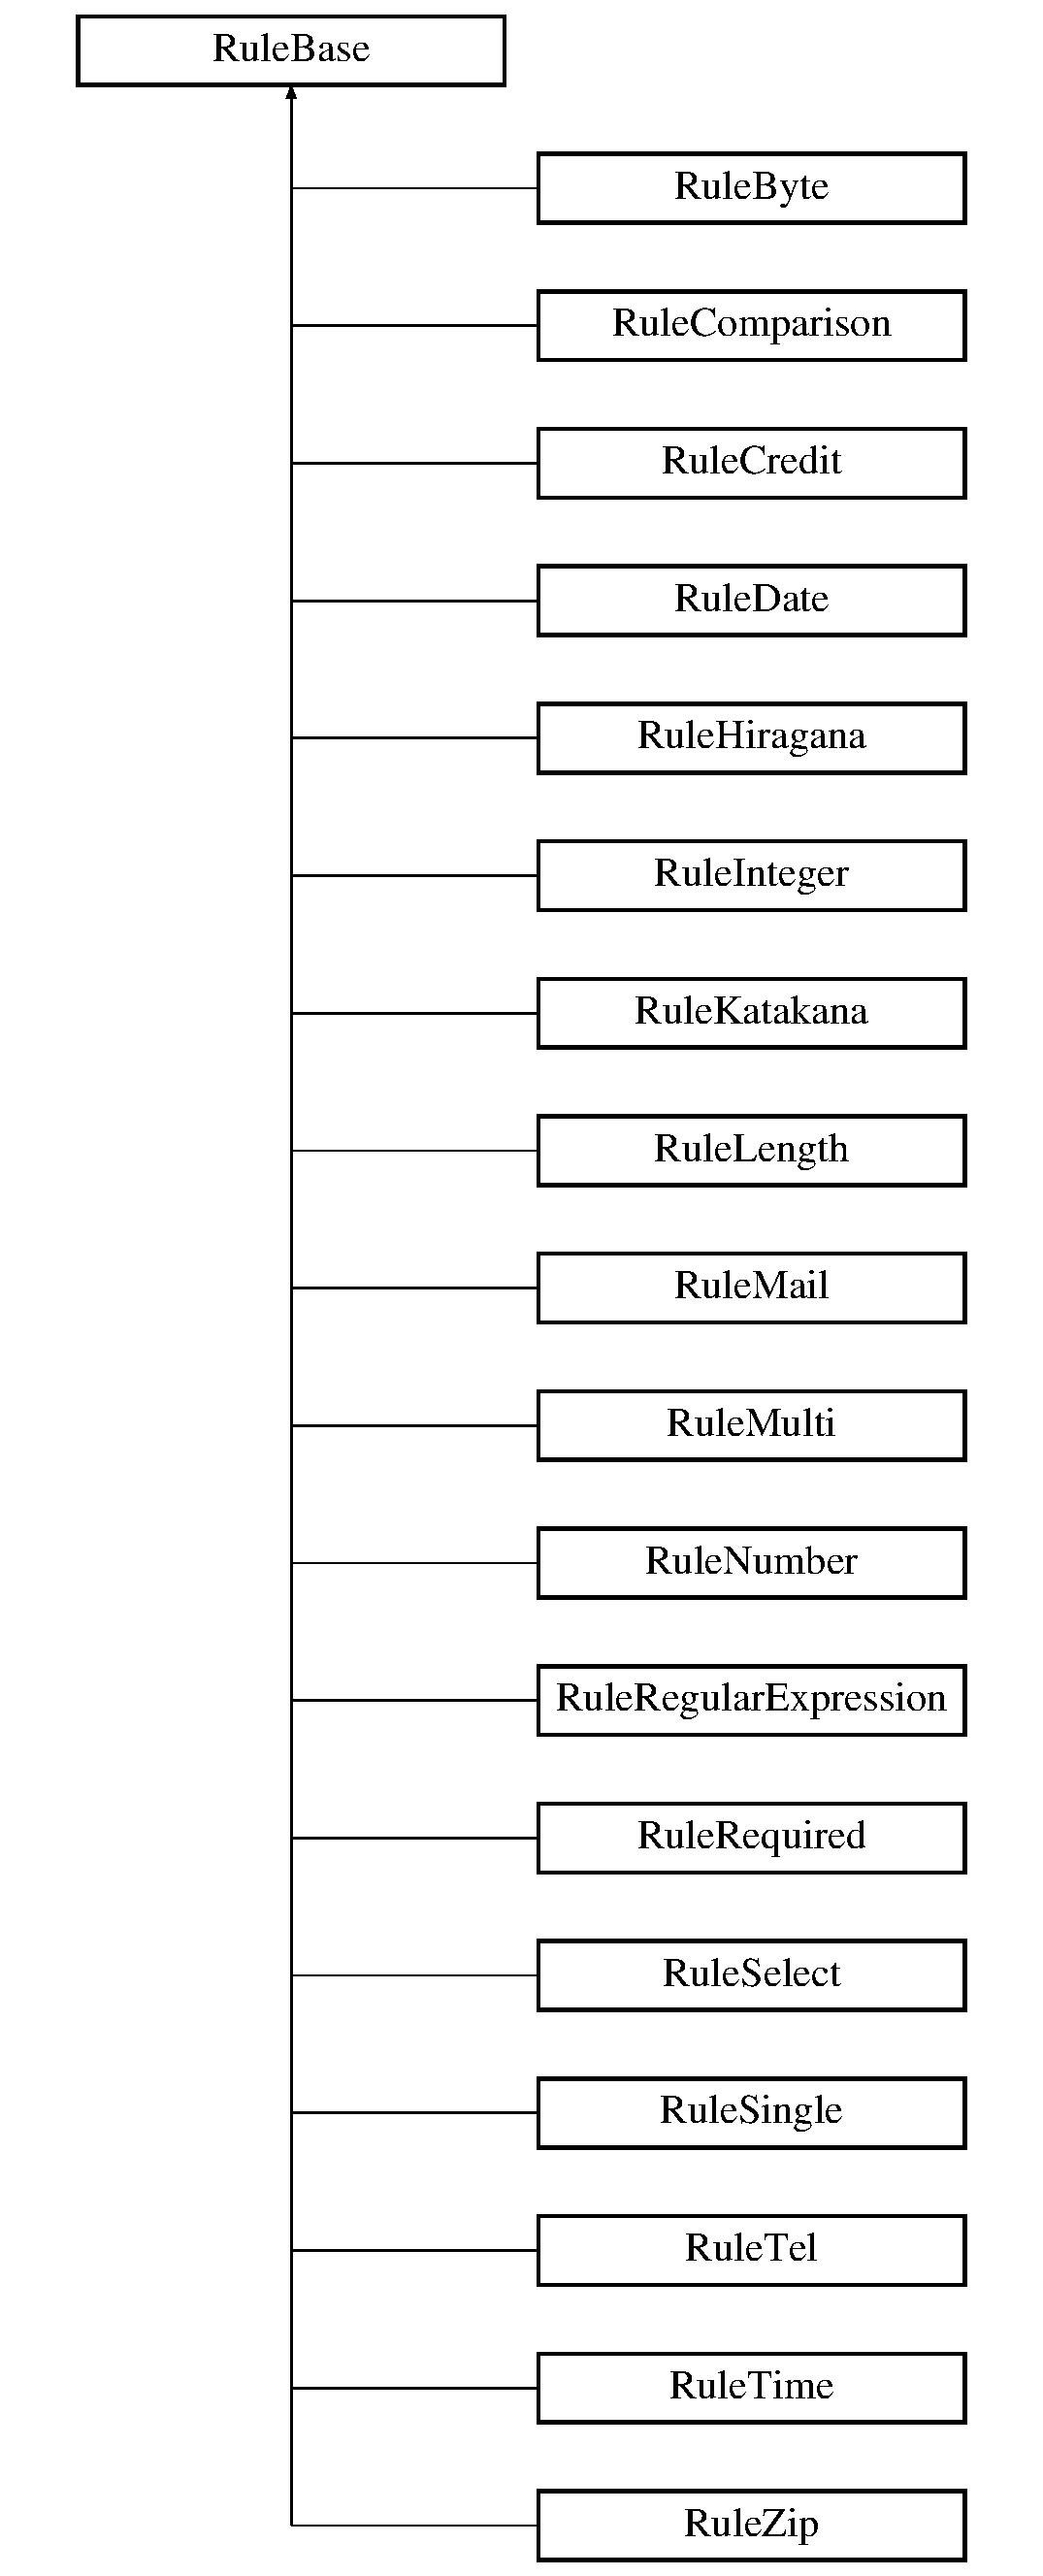
\includegraphics[height=12.000000cm]{class_rule_base}
\end{center}
\end{figure}
\subsection*{公開メンバ関数}
\begin{DoxyCompactItemize}
\item 
\hyperlink{class_rule_base_a7fdd69956610727a5a36b4f020bcf115}{\+\_\+\+\_\+construct} (\$file\+Nm)
\item 
\hyperlink{class_rule_base_a70eef3a06fda47704282eda5ea2706d9}{prepara} ()
\item 
\hyperlink{class_rule_base_afb0fafe7e02a3ae1993c01c19fad2bae}{run} ()
\end{DoxyCompactItemize}
\subsection*{フィールド}
\begin{DoxyCompactItemize}
\item 
\hypertarget{class_rule_base_a28d7688bd020a3b104adc19d1e08df96}{{\bfseries \$requests}}\label{class_rule_base_a28d7688bd020a3b104adc19d1e08df96}

\end{DoxyCompactItemize}
\subsection*{限定公開変数類}
\begin{DoxyCompactItemize}
\item 
\hypertarget{class_rule_base_a0f298096f322952a72a50f98a74c7b60}{{\bfseries \$value}}\label{class_rule_base_a0f298096f322952a72a50f98a74c7b60}

\item 
\hypertarget{class_rule_base_af24aefa35fa703a1521c8145fe8fa082}{{\bfseries \$infos}}\label{class_rule_base_af24aefa35fa703a1521c8145fe8fa082}

\item 
\hypertarget{class_rule_base_ab7baba555b2cbc79c5ff9ef47baee3d5}{{\bfseries \$inies}}\label{class_rule_base_ab7baba555b2cbc79c5ff9ef47baee3d5}

\end{DoxyCompactItemize}


\subsection{詳解}
基底ルールクラス

\begin{DoxyVersion}{バージョン}
1.\+0.\+0  U\+T\+F-\/8  2011/10/05  2011/10/19 
\end{DoxyVersion}
\begin{DoxyAuthor}{著者}
mamiya\+\_\+shou 
\end{DoxyAuthor}
\begin{DoxyCopyright}{著作権所有}
mamiya\+\_\+shou  M\+I\+T License  P\+H\+P 5.\+0 以上必須 
\end{DoxyCopyright}


\subsection{構築子と解体子}
\hypertarget{class_rule_base_a7fdd69956610727a5a36b4f020bcf115}{\index{Rule\+Base@{Rule\+Base}!\+\_\+\+\_\+construct@{\+\_\+\+\_\+construct}}
\index{\+\_\+\+\_\+construct@{\+\_\+\+\_\+construct}!Rule\+Base@{Rule\+Base}}
\subsubsection[{\+\_\+\+\_\+construct}]{\setlength{\rightskip}{0pt plus 5cm}\+\_\+\+\_\+construct (
\begin{DoxyParamCaption}
\item[{}]{\$file\+Nm}
\end{DoxyParamCaption}
)}}\label{class_rule_base_a7fdd69956610727a5a36b4f020bcf115}
コンストラクタ

public \begin{DoxyReturn}{戻り値}
void 
\end{DoxyReturn}


\subsection{関数詳解}
\hypertarget{class_rule_base_a70eef3a06fda47704282eda5ea2706d9}{\index{Rule\+Base@{Rule\+Base}!prepara@{prepara}}
\index{prepara@{prepara}!Rule\+Base@{Rule\+Base}}
\subsubsection[{prepara}]{\setlength{\rightskip}{0pt plus 5cm}prepara (
\begin{DoxyParamCaption}
{}
\end{DoxyParamCaption}
)}}\label{class_rule_base_a70eef3a06fda47704282eda5ea2706d9}
バリデーション準備

public 
\begin{DoxyParams}{引数}
{\em array} & 可変長引数 \\
\hline
\end{DoxyParams}
\begin{DoxyReturn}{戻り値}
void 
\end{DoxyReturn}
\hypertarget{class_rule_base_afb0fafe7e02a3ae1993c01c19fad2bae}{\index{Rule\+Base@{Rule\+Base}!run@{run}}
\index{run@{run}!Rule\+Base@{Rule\+Base}}
\subsubsection[{run}]{\setlength{\rightskip}{0pt plus 5cm}run (
\begin{DoxyParamCaption}
{}
\end{DoxyParamCaption}
)\hspace{0.3cm}{\ttfamily [abstract]}}}\label{class_rule_base_afb0fafe7e02a3ae1993c01c19fad2bae}
バリデートする

public  抽象メソッド 

このクラス詳解は次のファイルから抽出されました\+:\begin{DoxyCompactItemize}
\item 
Validate/rules/base\+\_\+rule.\+php\end{DoxyCompactItemize}

\hypertarget{class_rule_byte}{\section{Rule\+Byte クラス}
\label{class_rule_byte}\index{Rule\+Byte@{Rule\+Byte}}
}
Rule\+Byte の継承関係図\begin{figure}[H]
\begin{center}
\leavevmode
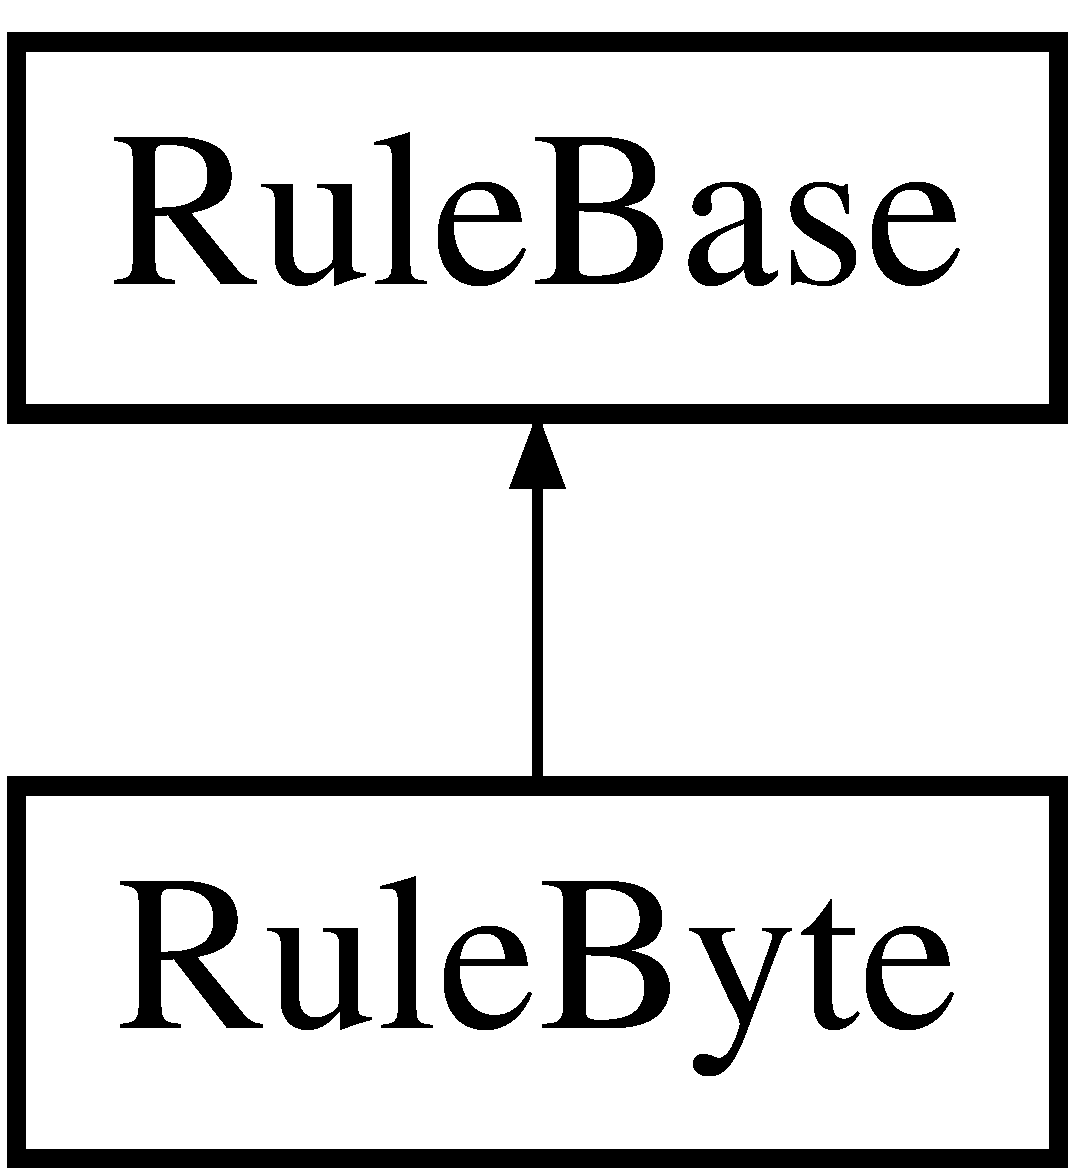
\includegraphics[height=2.000000cm]{class_rule_byte}
\end{center}
\end{figure}
\subsection*{公開メンバ関数}
\begin{DoxyCompactItemize}
\item 
\hyperlink{class_rule_byte_a095c5d389db211932136b53f25f39685}{\+\_\+\+\_\+construct} ()
\item 
\hyperlink{class_rule_byte_afb0fafe7e02a3ae1993c01c19fad2bae}{run} ()
\end{DoxyCompactItemize}
\subsection*{その他の継承メンバ}


\subsection{詳解}
ルール:バイト長クラス

\begin{DoxyVersion}{バージョン}
1.\+0.\+0  U\+T\+F-\/8  2011/10/05  2011/10/19 
\end{DoxyVersion}
\begin{DoxyAuthor}{著者}
mamiya\+\_\+shou 
\end{DoxyAuthor}
\begin{DoxyCopyright}{著作権所有}
mamiya\+\_\+shou  M\+I\+T License  P\+H\+P 5.\+0 以上必須 
\end{DoxyCopyright}


\subsection{構築子と解体子}
\hypertarget{class_rule_byte_a095c5d389db211932136b53f25f39685}{\index{Rule\+Byte@{Rule\+Byte}!\+\_\+\+\_\+construct@{\+\_\+\+\_\+construct}}
\index{\+\_\+\+\_\+construct@{\+\_\+\+\_\+construct}!Rule\+Byte@{Rule\+Byte}}
\subsubsection[{\+\_\+\+\_\+construct}]{\setlength{\rightskip}{0pt plus 5cm}\+\_\+\+\_\+construct (
\begin{DoxyParamCaption}
{}
\end{DoxyParamCaption}
)}}\label{class_rule_byte_a095c5d389db211932136b53f25f39685}
コンストラクタ

public \begin{DoxyReturn}{戻り値}
void 
\end{DoxyReturn}


\subsection{関数詳解}
\hypertarget{class_rule_byte_afb0fafe7e02a3ae1993c01c19fad2bae}{\index{Rule\+Byte@{Rule\+Byte}!run@{run}}
\index{run@{run}!Rule\+Byte@{Rule\+Byte}}
\subsubsection[{run}]{\setlength{\rightskip}{0pt plus 5cm}run (
\begin{DoxyParamCaption}
{}
\end{DoxyParamCaption}
)}}\label{class_rule_byte_afb0fafe7e02a3ae1993c01c19fad2bae}
バリデートする

public \begin{DoxyReturn}{戻り値}
boolean T\+R\+U\+E(\+O\+K) / string エラーメッセージ(\+N\+G) 
\end{DoxyReturn}

\begin{DoxyExceptions}{例外}
{\em Exception} & validate.\+php \hyperlink{class_rule_byte_afb0fafe7e02a3ae1993c01c19fad2bae}{run()}で捕捉する  未入力('')の場合は\+T\+R\+U\+Eを返す \\
\hline
\end{DoxyExceptions}


このクラス詳解は次のファイルから抽出されました\+:\begin{DoxyCompactItemize}
\item 
Validate/rules/byte.\+php\end{DoxyCompactItemize}

\hypertarget{class_rule_comparison}{\section{Rule\+Comparison クラス}
\label{class_rule_comparison}\index{Rule\+Comparison@{Rule\+Comparison}}
}
Rule\+Comparison の継承関係図\begin{figure}[H]
\begin{center}
\leavevmode
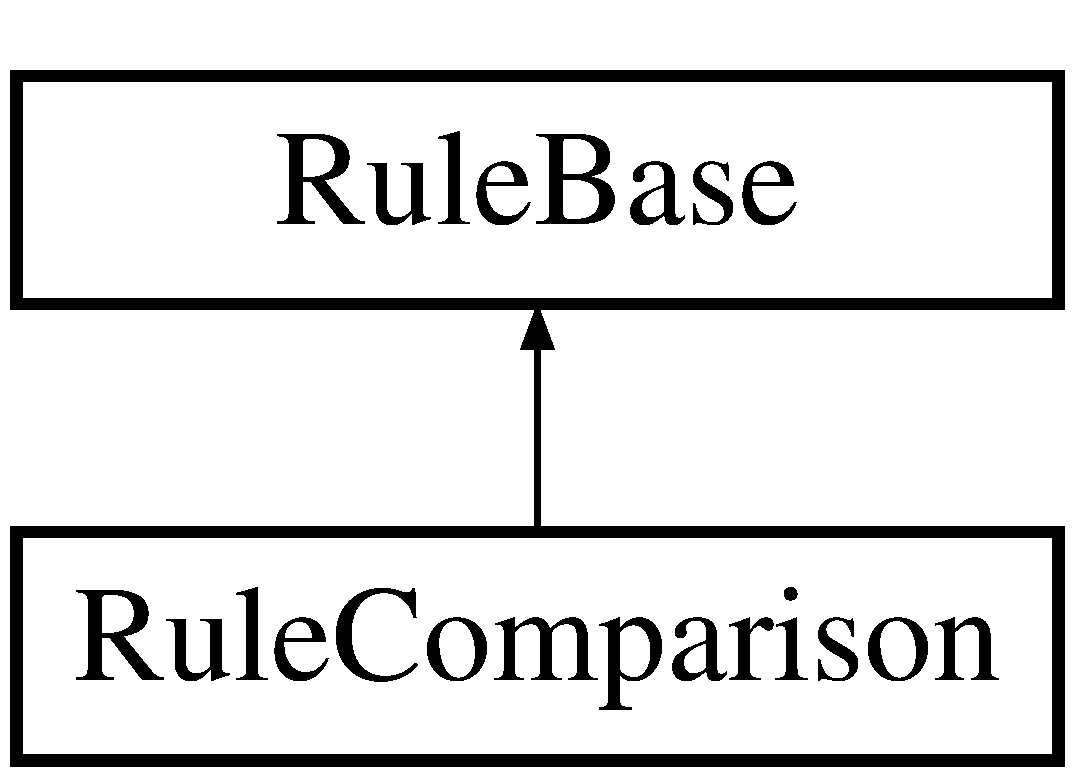
\includegraphics[height=2.000000cm]{class_rule_comparison}
\end{center}
\end{figure}
\subsection*{公開メンバ関数}
\begin{DoxyCompactItemize}
\item 
\hyperlink{class_rule_comparison_a095c5d389db211932136b53f25f39685}{\+\_\+\+\_\+construct} ()
\item 
\hyperlink{class_rule_comparison_afb0fafe7e02a3ae1993c01c19fad2bae}{run} ()
\end{DoxyCompactItemize}
\subsection*{その他の継承メンバ}


\subsection{詳解}
ルール:比較クラス

\begin{DoxyVersion}{バージョン}
1.\+0.\+0  U\+T\+F-\/8  2011/10/19  2011/10/19 
\end{DoxyVersion}
\begin{DoxyAuthor}{著者}
mamiya\+\_\+shou 
\end{DoxyAuthor}
\begin{DoxyCopyright}{著作権所有}
mamiya\+\_\+shou  M\+I\+T License  P\+H\+P 5.\+0 以上必須 
\end{DoxyCopyright}


\subsection{構築子と解体子}
\hypertarget{class_rule_comparison_a095c5d389db211932136b53f25f39685}{\index{Rule\+Comparison@{Rule\+Comparison}!\+\_\+\+\_\+construct@{\+\_\+\+\_\+construct}}
\index{\+\_\+\+\_\+construct@{\+\_\+\+\_\+construct}!Rule\+Comparison@{Rule\+Comparison}}
\subsubsection[{\+\_\+\+\_\+construct}]{\setlength{\rightskip}{0pt plus 5cm}\+\_\+\+\_\+construct (
\begin{DoxyParamCaption}
{}
\end{DoxyParamCaption}
)}}\label{class_rule_comparison_a095c5d389db211932136b53f25f39685}
コンストラクタ

public \begin{DoxyReturn}{戻り値}
void 
\end{DoxyReturn}


\subsection{関数詳解}
\hypertarget{class_rule_comparison_afb0fafe7e02a3ae1993c01c19fad2bae}{\index{Rule\+Comparison@{Rule\+Comparison}!run@{run}}
\index{run@{run}!Rule\+Comparison@{Rule\+Comparison}}
\subsubsection[{run}]{\setlength{\rightskip}{0pt plus 5cm}run (
\begin{DoxyParamCaption}
{}
\end{DoxyParamCaption}
)}}\label{class_rule_comparison_afb0fafe7e02a3ae1993c01c19fad2bae}
バリデートする

public \begin{DoxyReturn}{戻り値}
boolean T\+R\+U\+E(\+O\+K) / string エラーメッセージ(\+N\+G) 
\end{DoxyReturn}

\begin{DoxyExceptions}{例外}
{\em Exception} & validate.\+php \hyperlink{class_rule_comparison_afb0fafe7e02a3ae1993c01c19fad2bae}{run()}で捕捉する  全て未入力('')の場合は\+T\+R\+U\+Eを返す \\
\hline
\end{DoxyExceptions}


このクラス詳解は次のファイルから抽出されました\+:\begin{DoxyCompactItemize}
\item 
Validate/rules/comparison.\+php\end{DoxyCompactItemize}

\hypertarget{class_rule_credit}{\section{Rule\+Credit クラス}
\label{class_rule_credit}\index{Rule\+Credit@{Rule\+Credit}}
}
Rule\+Credit の継承関係図\begin{figure}[H]
\begin{center}
\leavevmode
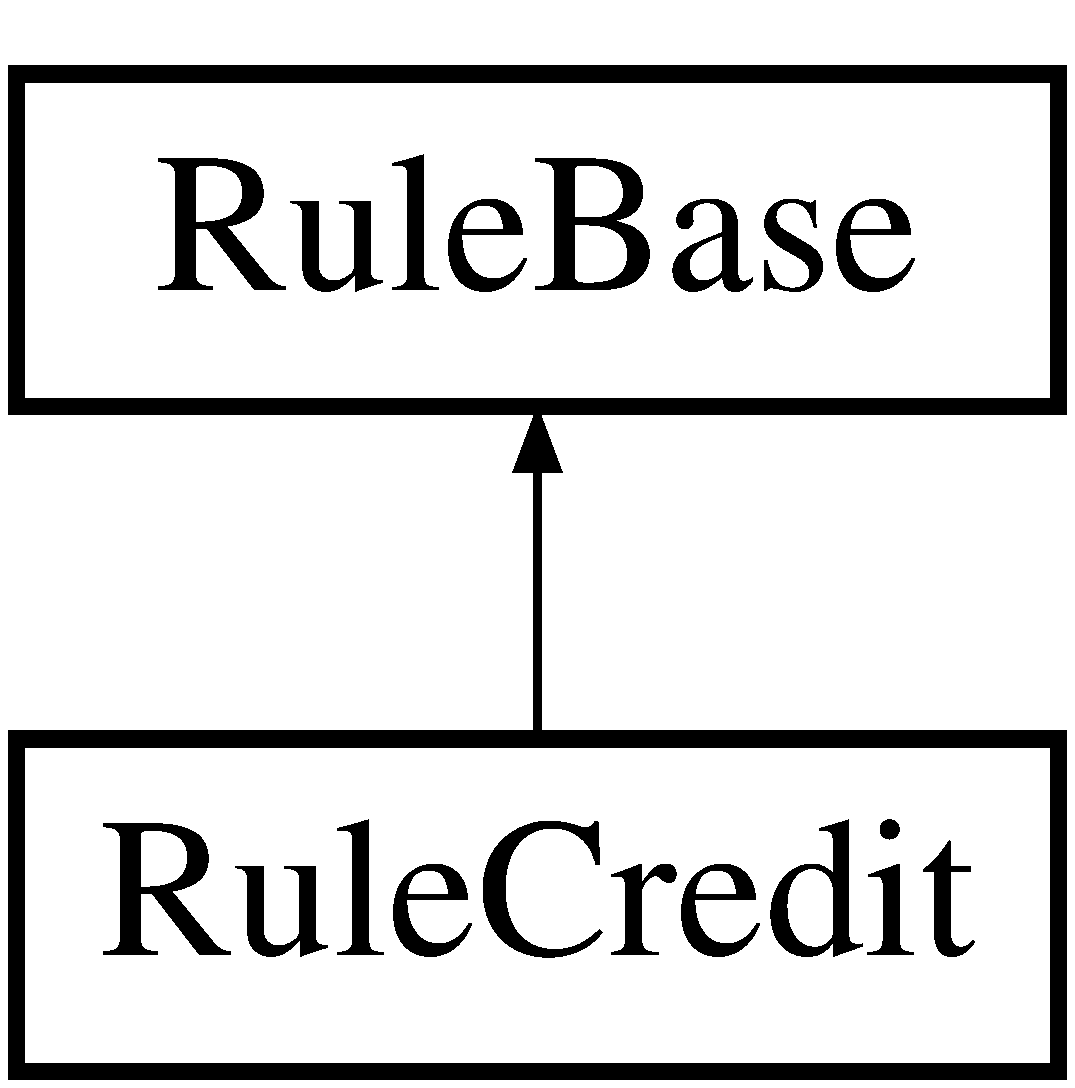
\includegraphics[height=2.000000cm]{class_rule_credit}
\end{center}
\end{figure}
\subsection*{公開メンバ関数}
\begin{DoxyCompactItemize}
\item 
\hyperlink{class_rule_credit_a095c5d389db211932136b53f25f39685}{\+\_\+\+\_\+construct} ()
\item 
\hyperlink{class_rule_credit_afb0fafe7e02a3ae1993c01c19fad2bae}{run} ()
\end{DoxyCompactItemize}
\subsection*{その他の継承メンバ}


\subsection{詳解}
ルール:クレジットカード番号クラス

\begin{DoxyVersion}{バージョン}
1.\+0.\+0  U\+T\+F-\/8  2011/10/10  2011/10/19 
\end{DoxyVersion}
\begin{DoxyAuthor}{著者}
mamiya\+\_\+shou 
\end{DoxyAuthor}
\begin{DoxyCopyright}{著作権所有}
mamiya\+\_\+shou  M\+I\+T License  P\+H\+P 5.\+0 以上必須 
\end{DoxyCopyright}


\subsection{構築子と解体子}
\hypertarget{class_rule_credit_a095c5d389db211932136b53f25f39685}{\index{Rule\+Credit@{Rule\+Credit}!\+\_\+\+\_\+construct@{\+\_\+\+\_\+construct}}
\index{\+\_\+\+\_\+construct@{\+\_\+\+\_\+construct}!Rule\+Credit@{Rule\+Credit}}
\subsubsection[{\+\_\+\+\_\+construct}]{\setlength{\rightskip}{0pt plus 5cm}\+\_\+\+\_\+construct (
\begin{DoxyParamCaption}
{}
\end{DoxyParamCaption}
)}}\label{class_rule_credit_a095c5d389db211932136b53f25f39685}
コンストラクタ

public \begin{DoxyReturn}{戻り値}
void 
\end{DoxyReturn}


\subsection{関数詳解}
\hypertarget{class_rule_credit_afb0fafe7e02a3ae1993c01c19fad2bae}{\index{Rule\+Credit@{Rule\+Credit}!run@{run}}
\index{run@{run}!Rule\+Credit@{Rule\+Credit}}
\subsubsection[{run}]{\setlength{\rightskip}{0pt plus 5cm}run (
\begin{DoxyParamCaption}
{}
\end{DoxyParamCaption}
)}}\label{class_rule_credit_afb0fafe7e02a3ae1993c01c19fad2bae}
バリデートする

public \begin{DoxyReturn}{戻り値}
boolean T\+R\+U\+E(\+O\+K) / string エラーメッセージ(\+N\+G)  未入力('')の場合は\+T\+R\+U\+Eを返す 
\end{DoxyReturn}


このクラス詳解は次のファイルから抽出されました\+:\begin{DoxyCompactItemize}
\item 
Validate/rules/credit.\+php\end{DoxyCompactItemize}

\hypertarget{class_rule_date}{\section{Rule\+Date クラス}
\label{class_rule_date}\index{Rule\+Date@{Rule\+Date}}
}
Rule\+Date の継承関係図\begin{figure}[H]
\begin{center}
\leavevmode
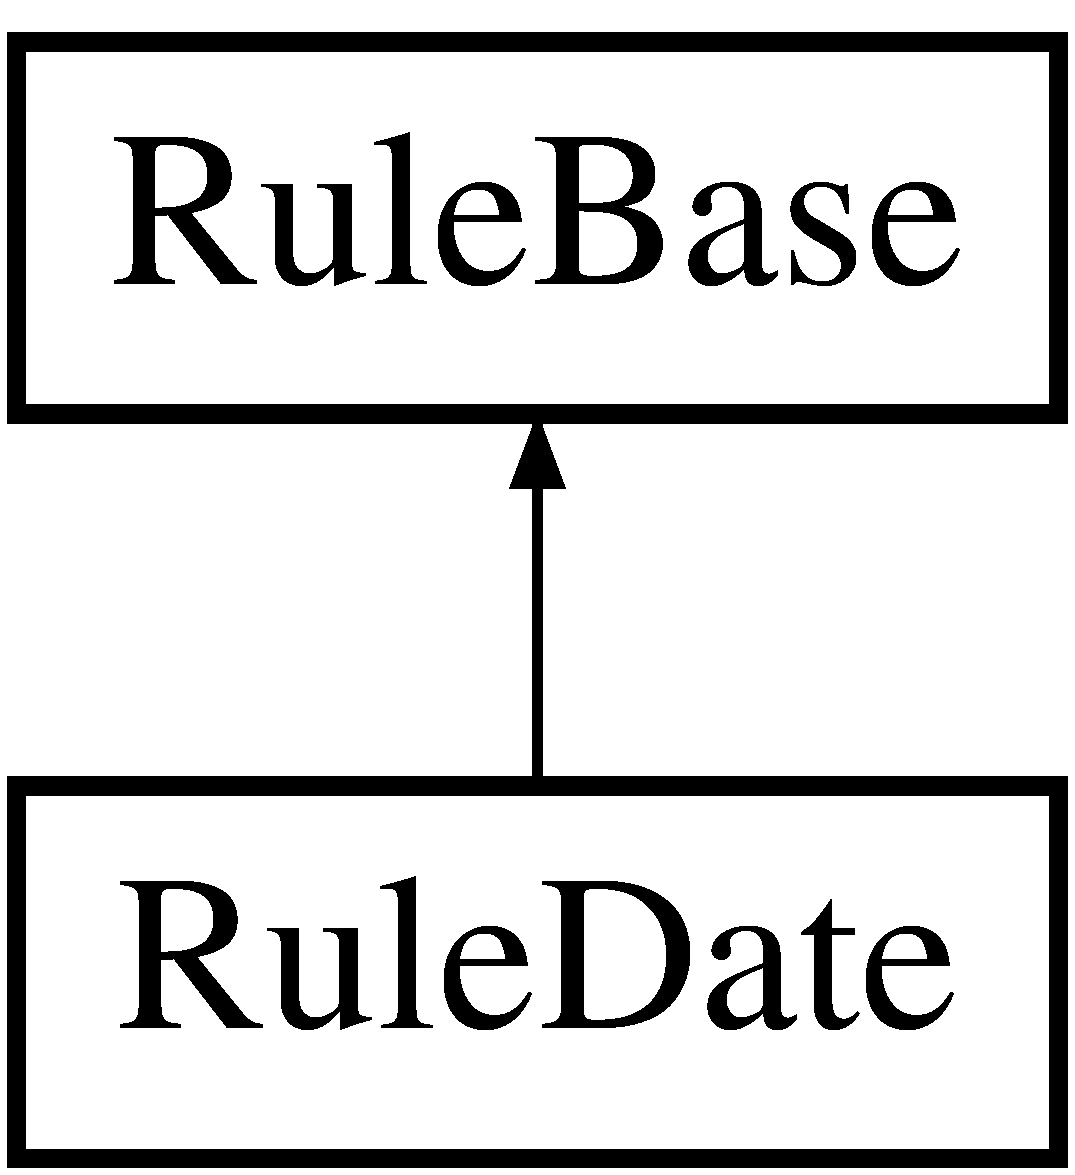
\includegraphics[height=2.000000cm]{class_rule_date}
\end{center}
\end{figure}
\subsection*{公開メンバ関数}
\begin{DoxyCompactItemize}
\item 
\hyperlink{class_rule_date_a095c5d389db211932136b53f25f39685}{\+\_\+\+\_\+construct} ()
\item 
\hyperlink{class_rule_date_afb0fafe7e02a3ae1993c01c19fad2bae}{run} ()
\end{DoxyCompactItemize}
\subsection*{その他の継承メンバ}


\subsection{詳解}
ルール:日付クラス

\begin{DoxyVersion}{バージョン}
1.\+0.\+0  U\+T\+F-\/8  2011/10/11  2011/10/19 
\end{DoxyVersion}
\begin{DoxyAuthor}{著者}
mamiya\+\_\+shou 
\end{DoxyAuthor}
\begin{DoxyCopyright}{著作権所有}
mamiya\+\_\+shou  M\+I\+T License  P\+H\+P 5.\+0 以上必須 
\end{DoxyCopyright}


\subsection{構築子と解体子}
\hypertarget{class_rule_date_a095c5d389db211932136b53f25f39685}{\index{Rule\+Date@{Rule\+Date}!\+\_\+\+\_\+construct@{\+\_\+\+\_\+construct}}
\index{\+\_\+\+\_\+construct@{\+\_\+\+\_\+construct}!Rule\+Date@{Rule\+Date}}
\subsubsection[{\+\_\+\+\_\+construct}]{\setlength{\rightskip}{0pt plus 5cm}\+\_\+\+\_\+construct (
\begin{DoxyParamCaption}
{}
\end{DoxyParamCaption}
)}}\label{class_rule_date_a095c5d389db211932136b53f25f39685}
コンストラクタ

public \begin{DoxyReturn}{戻り値}
void 
\end{DoxyReturn}


\subsection{関数詳解}
\hypertarget{class_rule_date_afb0fafe7e02a3ae1993c01c19fad2bae}{\index{Rule\+Date@{Rule\+Date}!run@{run}}
\index{run@{run}!Rule\+Date@{Rule\+Date}}
\subsubsection[{run}]{\setlength{\rightskip}{0pt plus 5cm}run (
\begin{DoxyParamCaption}
{}
\end{DoxyParamCaption}
)}}\label{class_rule_date_afb0fafe7e02a3ae1993c01c19fad2bae}
バリデートする

public \begin{DoxyReturn}{戻り値}
boolean T\+R\+U\+E(\+O\+K) / string エラーメッセージ(\+N\+G) 
\end{DoxyReturn}

\begin{DoxyExceptions}{例外}
{\em Exception} & validate.\+php \hyperlink{class_rule_date_afb0fafe7e02a3ae1993c01c19fad2bae}{run()}で捕捉する  未入力('')の場合は\+T\+R\+U\+Eを返す \\
\hline
\end{DoxyExceptions}


このクラス詳解は次のファイルから抽出されました\+:\begin{DoxyCompactItemize}
\item 
Validate/rules/date.\+php\end{DoxyCompactItemize}

\hypertarget{class_rule_hiragana}{\section{Rule\+Hiragana クラス}
\label{class_rule_hiragana}\index{Rule\+Hiragana@{Rule\+Hiragana}}
}
Rule\+Hiragana の継承関係図\begin{figure}[H]
\begin{center}
\leavevmode
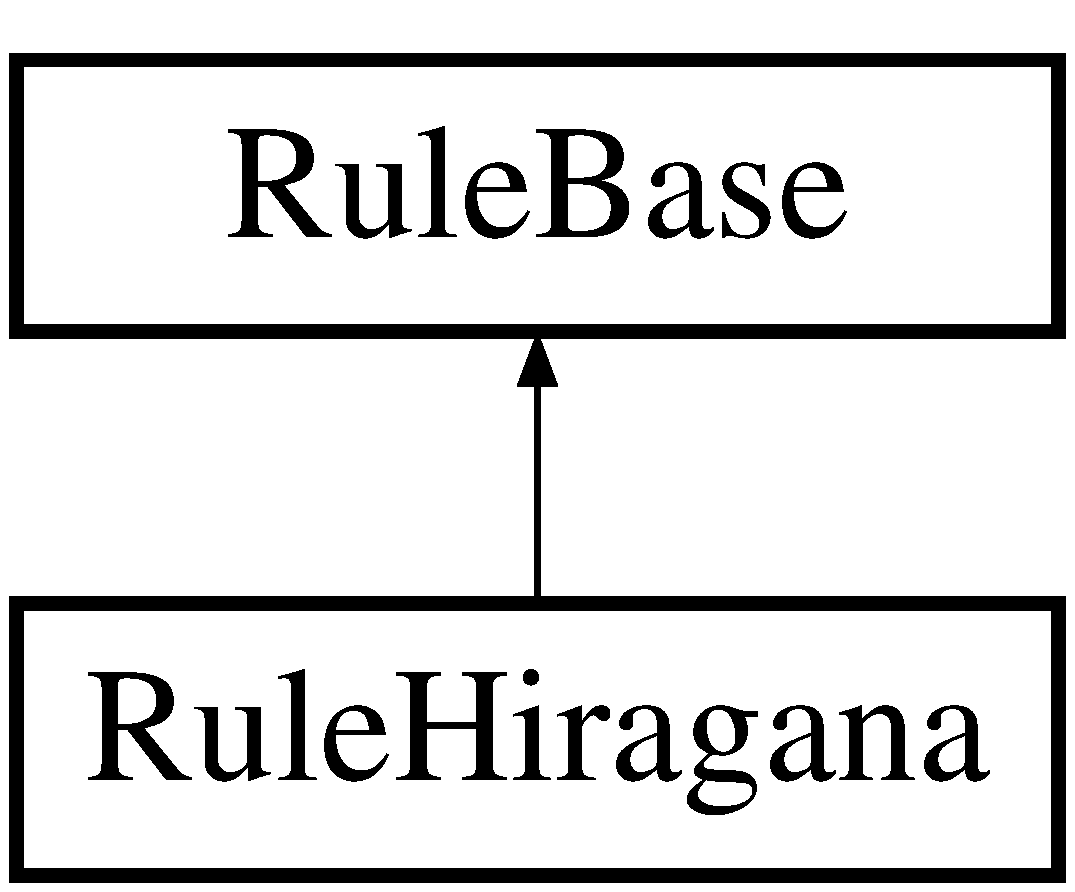
\includegraphics[height=2.000000cm]{class_rule_hiragana}
\end{center}
\end{figure}
\subsection*{公開メンバ関数}
\begin{DoxyCompactItemize}
\item 
\hyperlink{class_rule_hiragana_a095c5d389db211932136b53f25f39685}{\+\_\+\+\_\+construct} ()
\item 
\hyperlink{class_rule_hiragana_afb0fafe7e02a3ae1993c01c19fad2bae}{run} ()
\end{DoxyCompactItemize}
\subsection*{その他の継承メンバ}


\subsection{詳解}
ルール:ひらがなクラス

\begin{DoxyVersion}{バージョン}
1.\+0.\+0  U\+T\+F-\/8  2011/10/08  2011/10/19 
\end{DoxyVersion}
\begin{DoxyAuthor}{著者}
mamiya\+\_\+shou 
\end{DoxyAuthor}
\begin{DoxyCopyright}{著作権所有}
mamiya\+\_\+shou  M\+I\+T License  P\+H\+P 5.\+0 以上必須 
\end{DoxyCopyright}


\subsection{構築子と解体子}
\hypertarget{class_rule_hiragana_a095c5d389db211932136b53f25f39685}{\index{Rule\+Hiragana@{Rule\+Hiragana}!\+\_\+\+\_\+construct@{\+\_\+\+\_\+construct}}
\index{\+\_\+\+\_\+construct@{\+\_\+\+\_\+construct}!Rule\+Hiragana@{Rule\+Hiragana}}
\subsubsection[{\+\_\+\+\_\+construct}]{\setlength{\rightskip}{0pt plus 5cm}\+\_\+\+\_\+construct (
\begin{DoxyParamCaption}
{}
\end{DoxyParamCaption}
)}}\label{class_rule_hiragana_a095c5d389db211932136b53f25f39685}
コンストラクタ

public \begin{DoxyReturn}{戻り値}
void 
\end{DoxyReturn}


\subsection{関数詳解}
\hypertarget{class_rule_hiragana_afb0fafe7e02a3ae1993c01c19fad2bae}{\index{Rule\+Hiragana@{Rule\+Hiragana}!run@{run}}
\index{run@{run}!Rule\+Hiragana@{Rule\+Hiragana}}
\subsubsection[{run}]{\setlength{\rightskip}{0pt plus 5cm}run (
\begin{DoxyParamCaption}
{}
\end{DoxyParamCaption}
)}}\label{class_rule_hiragana_afb0fafe7e02a3ae1993c01c19fad2bae}
バリデートする

public \begin{DoxyReturn}{戻り値}
boolean T\+R\+U\+E(\+O\+K) / string エラーメッセージ(\+N\+G) 
\end{DoxyReturn}

\begin{DoxyExceptions}{例外}
{\em Exception} & validate.\+php \hyperlink{class_rule_hiragana_afb0fafe7e02a3ae1993c01c19fad2bae}{run()}で捕捉する  未入力('')の場合は\+T\+R\+U\+Eを返す  » \mbox{[}Code\+Igniter\mbox{]} Formバリデーションの拡張クラス Web Sytem $\vert$ A\+I\+D\+R\+E\+A\+M \href{http://blog.aidream.jp/codeigniter/codeigniter-form-validation-extend-class-1351.html}{\tt http\+://blog.\+aidream.\+jp/codeigniter/codeigniter-\/form-\/validation-\/extend-\/class-\/1351.\+html} \\
\hline
\end{DoxyExceptions}


このクラス詳解は次のファイルから抽出されました\+:\begin{DoxyCompactItemize}
\item 
Validate/rules/hiragana.\+php\end{DoxyCompactItemize}

\hypertarget{class_rule_integer}{\section{Rule\+Integer クラス}
\label{class_rule_integer}\index{Rule\+Integer@{Rule\+Integer}}
}
Rule\+Integer の継承関係図\begin{figure}[H]
\begin{center}
\leavevmode
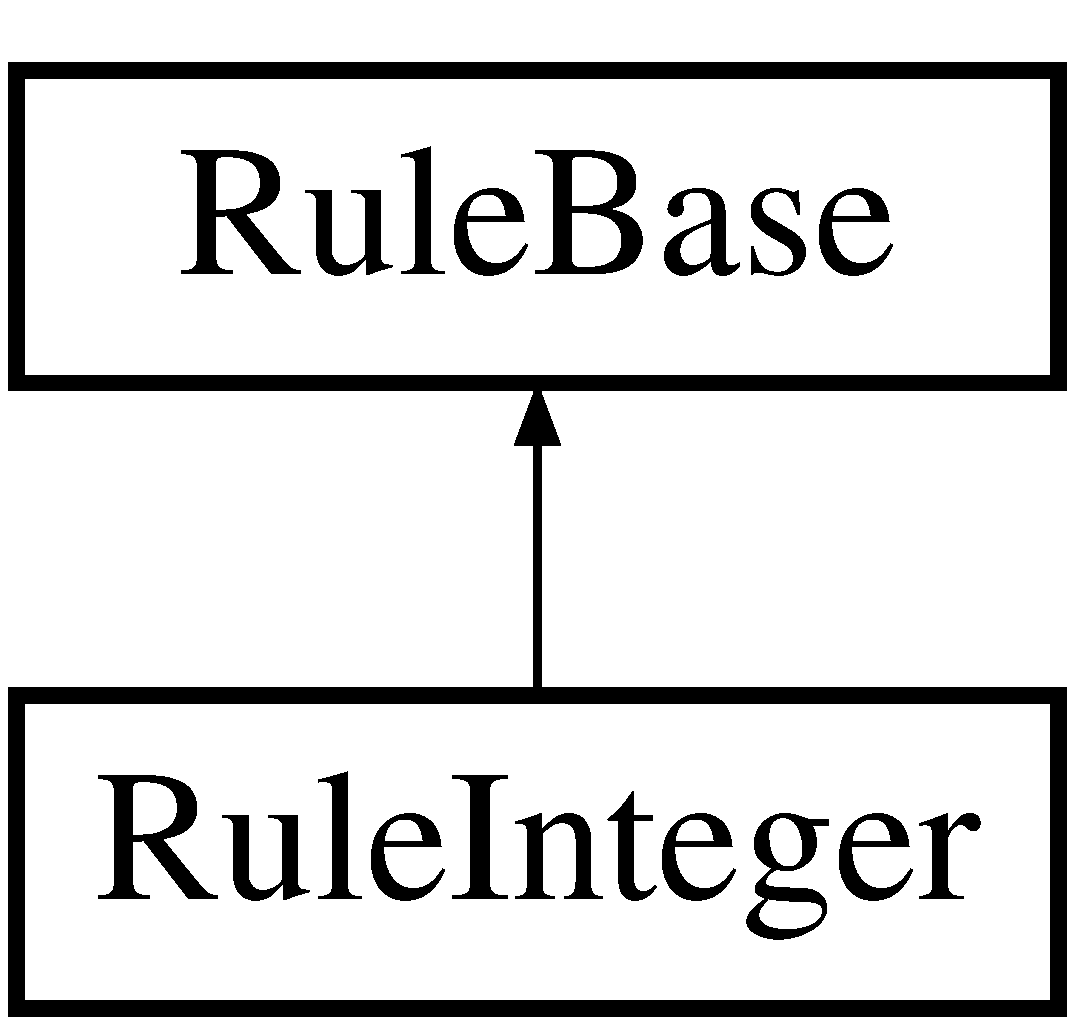
\includegraphics[height=2.000000cm]{class_rule_integer}
\end{center}
\end{figure}
\subsection*{公開メンバ関数}
\begin{DoxyCompactItemize}
\item 
\hyperlink{class_rule_integer_a095c5d389db211932136b53f25f39685}{\+\_\+\+\_\+construct} ()
\item 
\hyperlink{class_rule_integer_afb0fafe7e02a3ae1993c01c19fad2bae}{run} ()
\end{DoxyCompactItemize}
\subsection*{その他の継承メンバ}


\subsection{詳解}
ルール:整数クラス

\begin{DoxyVersion}{バージョン}
1.\+0.\+0  U\+T\+F-\/8  2011/10/06  2011/10/19 
\end{DoxyVersion}
\begin{DoxyAuthor}{著者}
mamiya\+\_\+shou 
\end{DoxyAuthor}
\begin{DoxyCopyright}{著作権所有}
mamiya\+\_\+shou  M\+I\+T License  P\+H\+P 5.\+0 以上必須 
\end{DoxyCopyright}


\subsection{構築子と解体子}
\hypertarget{class_rule_integer_a095c5d389db211932136b53f25f39685}{\index{Rule\+Integer@{Rule\+Integer}!\+\_\+\+\_\+construct@{\+\_\+\+\_\+construct}}
\index{\+\_\+\+\_\+construct@{\+\_\+\+\_\+construct}!Rule\+Integer@{Rule\+Integer}}
\subsubsection[{\+\_\+\+\_\+construct}]{\setlength{\rightskip}{0pt plus 5cm}\+\_\+\+\_\+construct (
\begin{DoxyParamCaption}
{}
\end{DoxyParamCaption}
)}}\label{class_rule_integer_a095c5d389db211932136b53f25f39685}
コンストラクタ

public \begin{DoxyReturn}{戻り値}
void 
\end{DoxyReturn}


\subsection{関数詳解}
\hypertarget{class_rule_integer_afb0fafe7e02a3ae1993c01c19fad2bae}{\index{Rule\+Integer@{Rule\+Integer}!run@{run}}
\index{run@{run}!Rule\+Integer@{Rule\+Integer}}
\subsubsection[{run}]{\setlength{\rightskip}{0pt plus 5cm}run (
\begin{DoxyParamCaption}
{}
\end{DoxyParamCaption}
)}}\label{class_rule_integer_afb0fafe7e02a3ae1993c01c19fad2bae}
バリデートする

public \begin{DoxyReturn}{戻り値}
boolean T\+R\+U\+E(\+O\+K) / string エラーメッセージ(\+N\+G)  未入力('')の場合は\+T\+R\+U\+Eを返す 
\end{DoxyReturn}


このクラス詳解は次のファイルから抽出されました\+:\begin{DoxyCompactItemize}
\item 
Validate/rules/integer.\+php\end{DoxyCompactItemize}

\hypertarget{class_rule_katakana}{\section{Rule\+Katakana クラス}
\label{class_rule_katakana}\index{Rule\+Katakana@{Rule\+Katakana}}
}
Rule\+Katakana の継承関係図\begin{figure}[H]
\begin{center}
\leavevmode
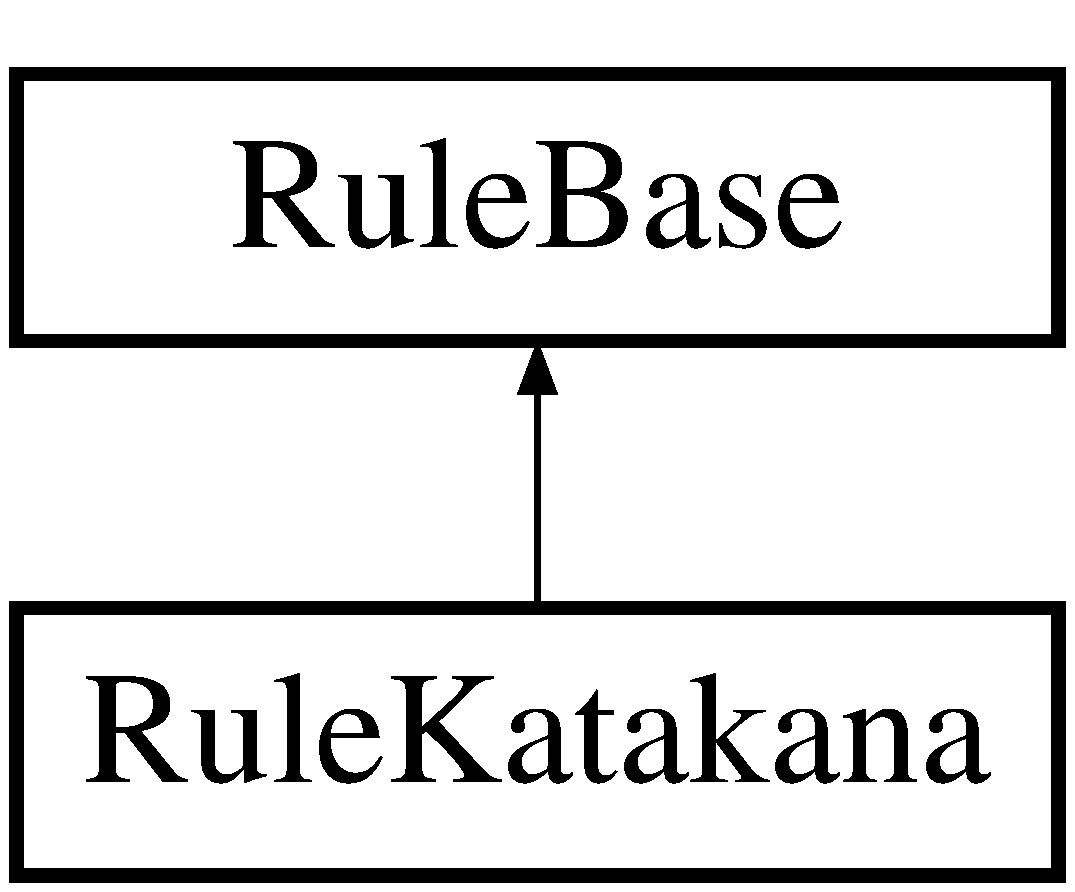
\includegraphics[height=2.000000cm]{class_rule_katakana}
\end{center}
\end{figure}
\subsection*{公開メンバ関数}
\begin{DoxyCompactItemize}
\item 
\hyperlink{class_rule_katakana_a095c5d389db211932136b53f25f39685}{\+\_\+\+\_\+construct} ()
\item 
\hyperlink{class_rule_katakana_afb0fafe7e02a3ae1993c01c19fad2bae}{run} ()
\end{DoxyCompactItemize}
\subsection*{その他の継承メンバ}


\subsection{詳解}
ルール:カタカナクラス

\begin{DoxyVersion}{バージョン}
1.\+0.\+0  U\+T\+F-\/8  2011/10/09  2011/10/19 
\end{DoxyVersion}
\begin{DoxyAuthor}{著者}
mamiya\+\_\+shou 
\end{DoxyAuthor}
\begin{DoxyCopyright}{著作権所有}
mamiya\+\_\+shou  M\+I\+T License  P\+H\+P 5.\+0 以上必須 
\end{DoxyCopyright}


\subsection{構築子と解体子}
\hypertarget{class_rule_katakana_a095c5d389db211932136b53f25f39685}{\index{Rule\+Katakana@{Rule\+Katakana}!\+\_\+\+\_\+construct@{\+\_\+\+\_\+construct}}
\index{\+\_\+\+\_\+construct@{\+\_\+\+\_\+construct}!Rule\+Katakana@{Rule\+Katakana}}
\subsubsection[{\+\_\+\+\_\+construct}]{\setlength{\rightskip}{0pt plus 5cm}\+\_\+\+\_\+construct (
\begin{DoxyParamCaption}
{}
\end{DoxyParamCaption}
)}}\label{class_rule_katakana_a095c5d389db211932136b53f25f39685}
コンストラクタ

public \begin{DoxyReturn}{戻り値}
void 
\end{DoxyReturn}


\subsection{関数詳解}
\hypertarget{class_rule_katakana_afb0fafe7e02a3ae1993c01c19fad2bae}{\index{Rule\+Katakana@{Rule\+Katakana}!run@{run}}
\index{run@{run}!Rule\+Katakana@{Rule\+Katakana}}
\subsubsection[{run}]{\setlength{\rightskip}{0pt plus 5cm}run (
\begin{DoxyParamCaption}
{}
\end{DoxyParamCaption}
)}}\label{class_rule_katakana_afb0fafe7e02a3ae1993c01c19fad2bae}
バリデートする

public \begin{DoxyReturn}{戻り値}
boolean T\+R\+U\+E(\+O\+K) / string エラーメッセージ(\+N\+G) 
\end{DoxyReturn}

\begin{DoxyExceptions}{例外}
{\em Exception} & validate.\+php \hyperlink{class_rule_katakana_afb0fafe7e02a3ae1993c01c19fad2bae}{run()}で捕捉する  未入力('')の場合は\+T\+R\+U\+Eを返す  » \mbox{[}Code\+Igniter\mbox{]} Formバリデーションの拡張クラス Web Sytem $\vert$ A\+I\+D\+R\+E\+A\+M \href{http://blog.aidream.jp/codeigniter/codeigniter-form-validation-extend-class-1351.html}{\tt http\+://blog.\+aidream.\+jp/codeigniter/codeigniter-\/form-\/validation-\/extend-\/class-\/1351.\+html} \\
\hline
\end{DoxyExceptions}


このクラス詳解は次のファイルから抽出されました\+:\begin{DoxyCompactItemize}
\item 
Validate/rules/katakana.\+php\end{DoxyCompactItemize}

\hypertarget{class_rule_length}{\section{Rule\+Length クラス}
\label{class_rule_length}\index{Rule\+Length@{Rule\+Length}}
}
Rule\+Length の継承関係図\begin{figure}[H]
\begin{center}
\leavevmode
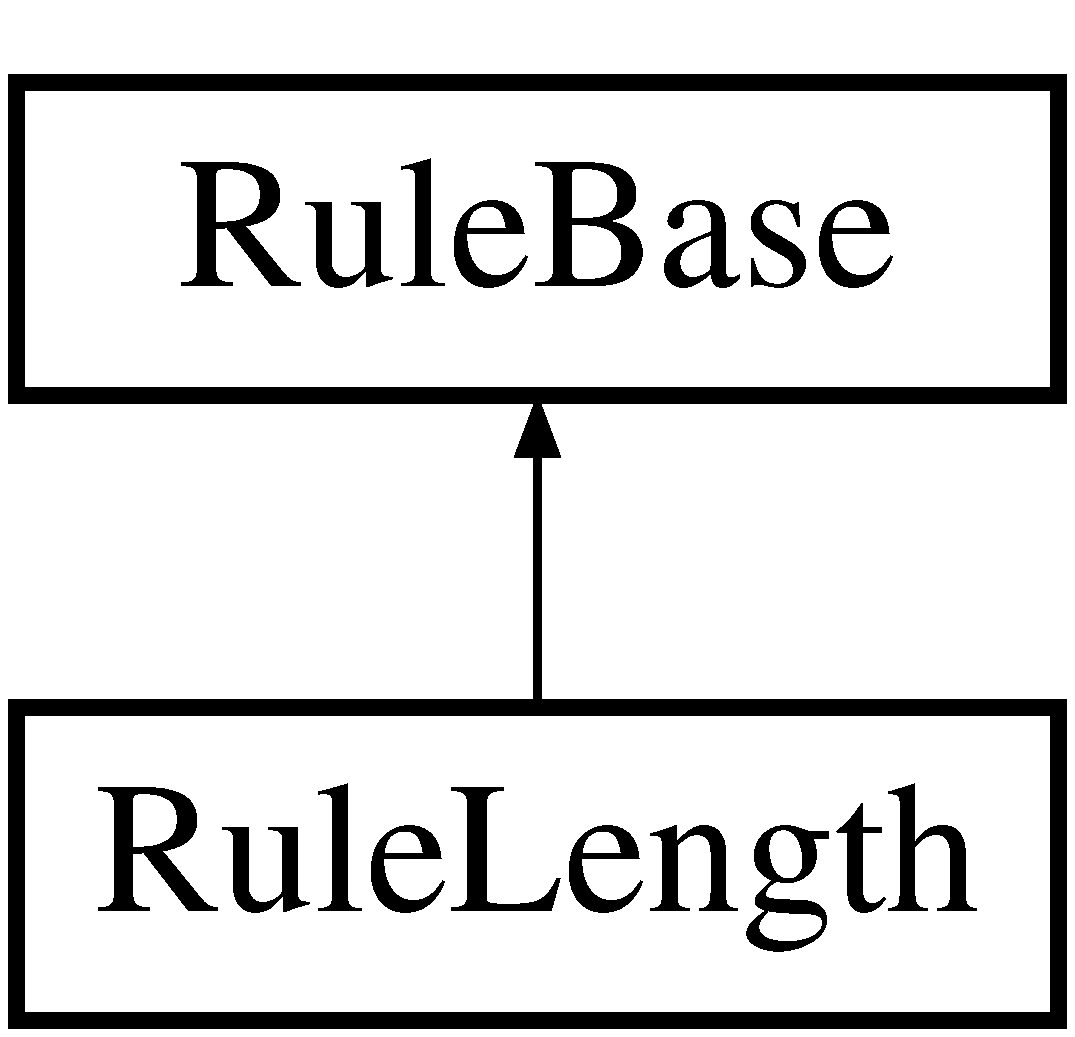
\includegraphics[height=2.000000cm]{class_rule_length}
\end{center}
\end{figure}
\subsection*{公開メンバ関数}
\begin{DoxyCompactItemize}
\item 
\hyperlink{class_rule_length_a095c5d389db211932136b53f25f39685}{\+\_\+\+\_\+construct} ()
\item 
\hyperlink{class_rule_length_afb0fafe7e02a3ae1993c01c19fad2bae}{run} ()
\end{DoxyCompactItemize}
\subsection*{その他の継承メンバ}


\subsection{詳解}
ルール:文字長クラス

\begin{DoxyVersion}{バージョン}
1.\+0.\+0  U\+T\+F-\/8  2011/10/05  2011/10/19 
\end{DoxyVersion}
\begin{DoxyAuthor}{著者}
mamiya\+\_\+shou 
\end{DoxyAuthor}
\begin{DoxyCopyright}{著作権所有}
mamiya\+\_\+shou  M\+I\+T License 
\end{DoxyCopyright}


\subsection{構築子と解体子}
\hypertarget{class_rule_length_a095c5d389db211932136b53f25f39685}{\index{Rule\+Length@{Rule\+Length}!\+\_\+\+\_\+construct@{\+\_\+\+\_\+construct}}
\index{\+\_\+\+\_\+construct@{\+\_\+\+\_\+construct}!Rule\+Length@{Rule\+Length}}
\subsubsection[{\+\_\+\+\_\+construct}]{\setlength{\rightskip}{0pt plus 5cm}\+\_\+\+\_\+construct (
\begin{DoxyParamCaption}
{}
\end{DoxyParamCaption}
)}}\label{class_rule_length_a095c5d389db211932136b53f25f39685}
コンストラクタ

public \begin{DoxyReturn}{戻り値}
void 
\end{DoxyReturn}


\subsection{関数詳解}
\hypertarget{class_rule_length_afb0fafe7e02a3ae1993c01c19fad2bae}{\index{Rule\+Length@{Rule\+Length}!run@{run}}
\index{run@{run}!Rule\+Length@{Rule\+Length}}
\subsubsection[{run}]{\setlength{\rightskip}{0pt plus 5cm}run (
\begin{DoxyParamCaption}
{}
\end{DoxyParamCaption}
)}}\label{class_rule_length_afb0fafe7e02a3ae1993c01c19fad2bae}
バリデートする

public \begin{DoxyReturn}{戻り値}
boolean T\+R\+U\+E(\+O\+K) / string エラーメッセージ(\+N\+G) 
\end{DoxyReturn}

\begin{DoxyExceptions}{例外}
{\em Exception} & validate.\+php \hyperlink{class_rule_length_afb0fafe7e02a3ae1993c01c19fad2bae}{run()}で捕捉する  未入力('')の場合は\+T\+R\+U\+Eを返す \\
\hline
\end{DoxyExceptions}


このクラス詳解は次のファイルから抽出されました\+:\begin{DoxyCompactItemize}
\item 
Validate/rules/length.\+php\end{DoxyCompactItemize}

\hypertarget{class_rule_mail}{\section{Rule\+Mail クラス}
\label{class_rule_mail}\index{Rule\+Mail@{Rule\+Mail}}
}
Rule\+Mail の継承関係図\begin{figure}[H]
\begin{center}
\leavevmode
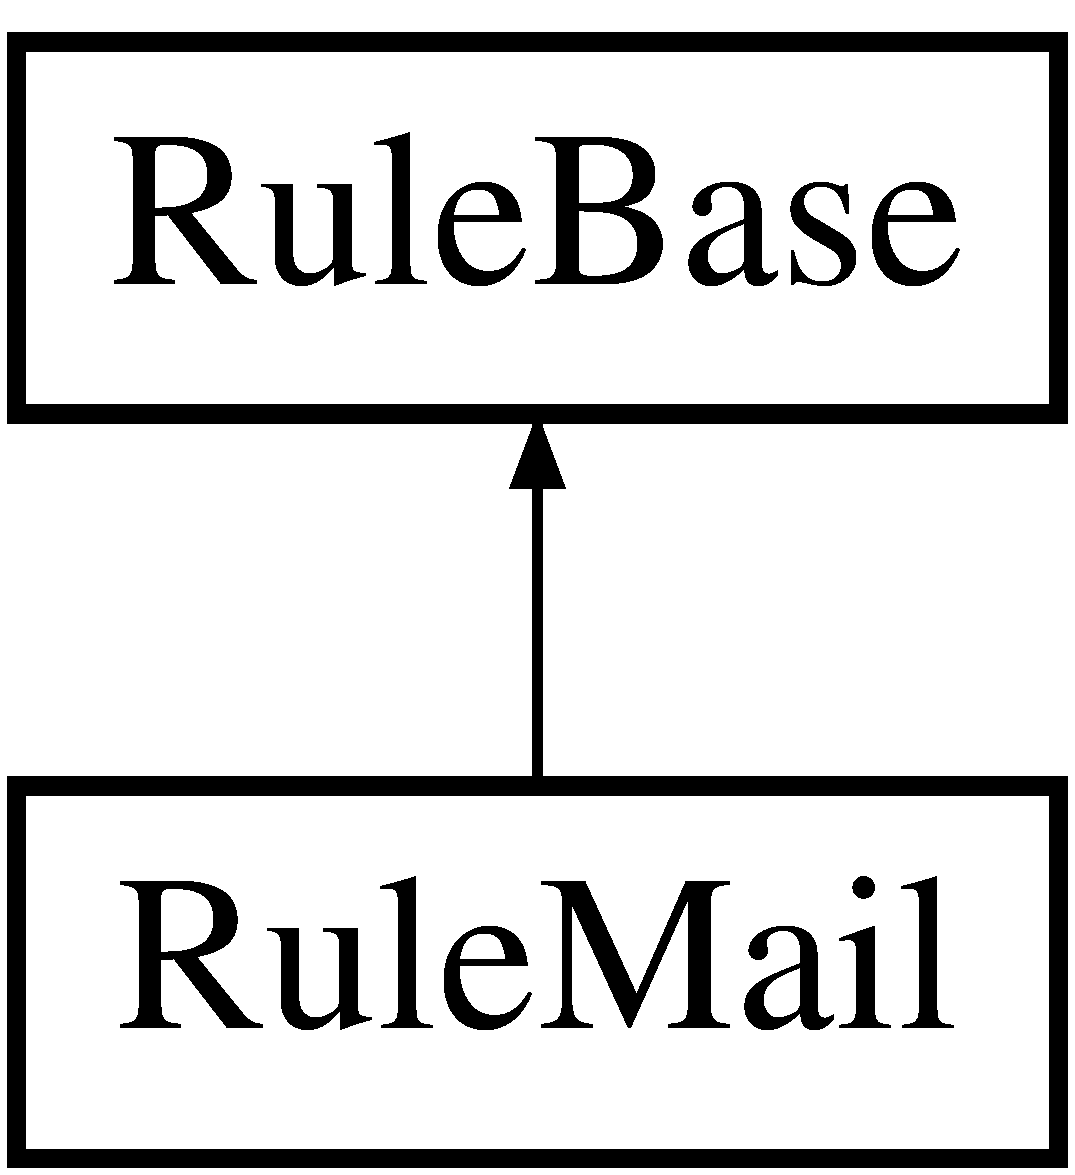
\includegraphics[height=2.000000cm]{class_rule_mail}
\end{center}
\end{figure}
\subsection*{公開メンバ関数}
\begin{DoxyCompactItemize}
\item 
\hyperlink{class_rule_mail_a095c5d389db211932136b53f25f39685}{\+\_\+\+\_\+construct} ()
\item 
\hyperlink{class_rule_mail_afb0fafe7e02a3ae1993c01c19fad2bae}{run} ()
\end{DoxyCompactItemize}
\subsection*{フィールド}
\begin{DoxyCompactItemize}
\item 
\hypertarget{class_rule_mail_ae120b9206d39e1922b268a74697c4775}{const {\bfseries M\+A\+I\+L\+\_\+\+P\+A\+T\+T\+E\+R\+N} = '/$^\wedge$(\mbox{[}a-\/z0-\/9\+\_\+\mbox{]}$\vert$\textbackslash{}-\/$\vert$\textbackslash{}.$\vert$\textbackslash{}+)+@((\mbox{[}a-\/z0-\/9\+\_\+\mbox{]}$\vert$\textbackslash{}-\/)+\textbackslash{}.)+\mbox{[}a-\/z\mbox{]}\{2,6\}\$/i'}\label{class_rule_mail_ae120b9206d39e1922b268a74697c4775}

\end{DoxyCompactItemize}
\subsection*{その他の継承メンバ}


\subsection{詳解}
ルール:メールアドレスクラス

\begin{DoxyVersion}{バージョン}
1.\+0.\+0  U\+T\+F-\/8  2011/10/09  2011/10/19 
\end{DoxyVersion}
\begin{DoxyAuthor}{著者}
mamiya\+\_\+shou 
\end{DoxyAuthor}
\begin{DoxyCopyright}{著作権所有}
mamiya\+\_\+shou  M\+I\+T License  P\+H\+P 5.\+0 以上必須 
\end{DoxyCopyright}


\subsection{構築子と解体子}
\hypertarget{class_rule_mail_a095c5d389db211932136b53f25f39685}{\index{Rule\+Mail@{Rule\+Mail}!\+\_\+\+\_\+construct@{\+\_\+\+\_\+construct}}
\index{\+\_\+\+\_\+construct@{\+\_\+\+\_\+construct}!Rule\+Mail@{Rule\+Mail}}
\subsubsection[{\+\_\+\+\_\+construct}]{\setlength{\rightskip}{0pt plus 5cm}\+\_\+\+\_\+construct (
\begin{DoxyParamCaption}
{}
\end{DoxyParamCaption}
)}}\label{class_rule_mail_a095c5d389db211932136b53f25f39685}
コンストラクタ

public \begin{DoxyReturn}{戻り値}
void 
\end{DoxyReturn}


\subsection{関数詳解}
\hypertarget{class_rule_mail_afb0fafe7e02a3ae1993c01c19fad2bae}{\index{Rule\+Mail@{Rule\+Mail}!run@{run}}
\index{run@{run}!Rule\+Mail@{Rule\+Mail}}
\subsubsection[{run}]{\setlength{\rightskip}{0pt plus 5cm}run (
\begin{DoxyParamCaption}
{}
\end{DoxyParamCaption}
)}}\label{class_rule_mail_afb0fafe7e02a3ae1993c01c19fad2bae}
バリデートする

public \begin{DoxyReturn}{戻り値}
boolean T\+R\+U\+E(\+O\+K) / string エラーメッセージ(\+N\+G)  未入力('')の場合は\+T\+R\+U\+Eを返す  re\+: P\+H\+Pでメールアドレスかどうか調べる方法 (ハズレ日記) \href{http://catbot.net/blog/2007/06/re_php.html}{\tt http\+://catbot.\+net/blog/2007/06/re\+\_\+php.\+html} 
\end{DoxyReturn}


このクラス詳解は次のファイルから抽出されました\+:\begin{DoxyCompactItemize}
\item 
Validate/rules/mail.\+php\end{DoxyCompactItemize}

\hypertarget{class_rule_multi}{\section{Rule\+Multi クラス}
\label{class_rule_multi}\index{Rule\+Multi@{Rule\+Multi}}
}
Rule\+Multi の継承関係図\begin{figure}[H]
\begin{center}
\leavevmode
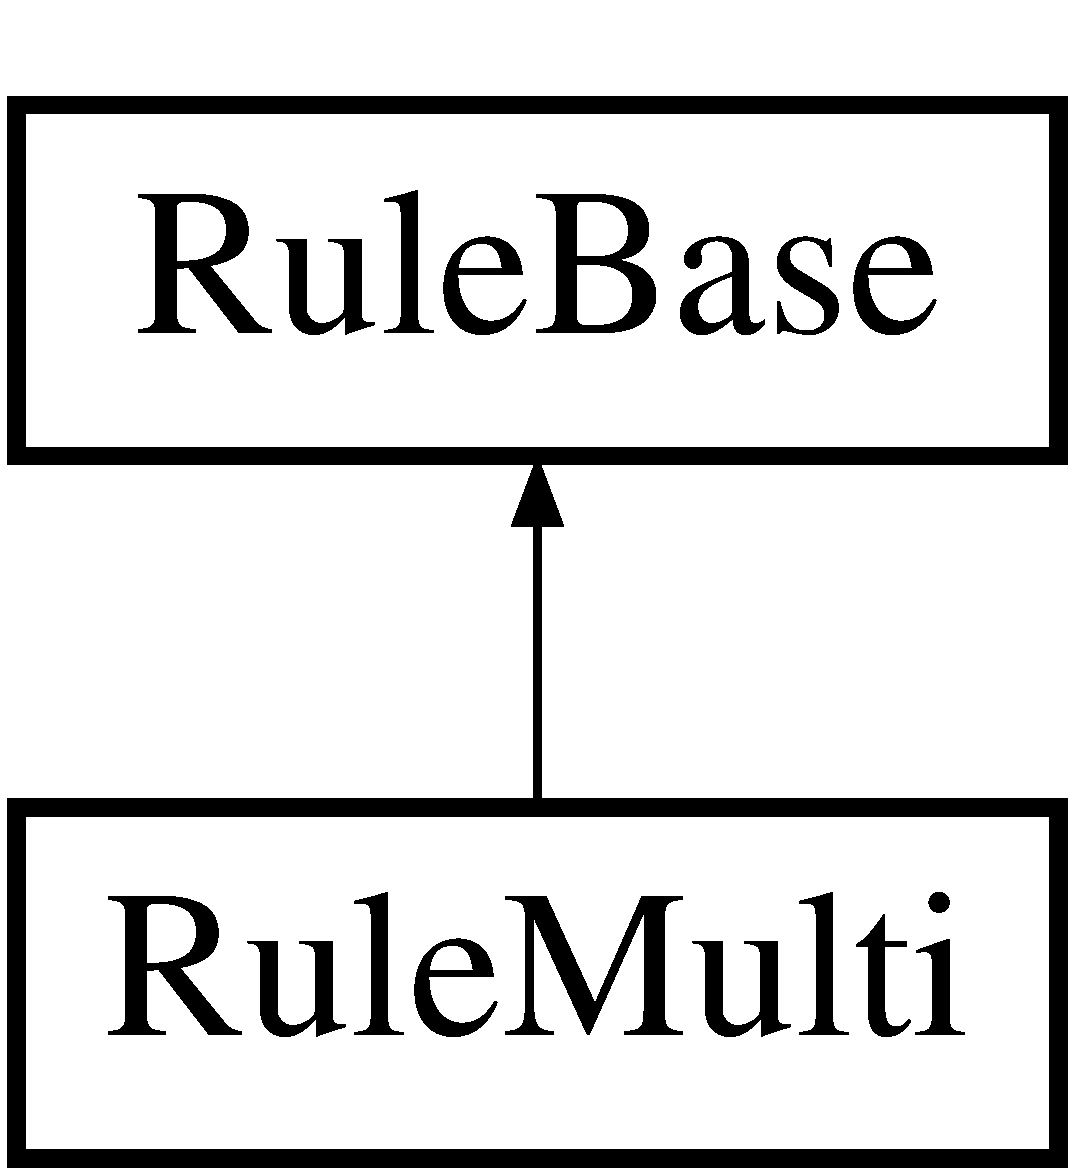
\includegraphics[height=2.000000cm]{class_rule_multi}
\end{center}
\end{figure}
\subsection*{公開メンバ関数}
\begin{DoxyCompactItemize}
\item 
\hyperlink{class_rule_multi_a095c5d389db211932136b53f25f39685}{\+\_\+\+\_\+construct} ()
\item 
\hyperlink{class_rule_multi_afb0fafe7e02a3ae1993c01c19fad2bae}{run} ()
\end{DoxyCompactItemize}
\subsection*{その他の継承メンバ}


\subsection{詳解}
ルール:全角文字クラス

\begin{DoxyVersion}{バージョン}
1.\+0.\+0  U\+T\+F-\/8  2011/10/08  2011/10/19 
\end{DoxyVersion}
\begin{DoxyAuthor}{著者}
mamiya\+\_\+shou 
\end{DoxyAuthor}
\begin{DoxyCopyright}{著作権所有}
mamiya\+\_\+shou  M\+I\+T License  P\+H\+P 5.\+0 以上必須 
\end{DoxyCopyright}


\subsection{構築子と解体子}
\hypertarget{class_rule_multi_a095c5d389db211932136b53f25f39685}{\index{Rule\+Multi@{Rule\+Multi}!\+\_\+\+\_\+construct@{\+\_\+\+\_\+construct}}
\index{\+\_\+\+\_\+construct@{\+\_\+\+\_\+construct}!Rule\+Multi@{Rule\+Multi}}
\subsubsection[{\+\_\+\+\_\+construct}]{\setlength{\rightskip}{0pt plus 5cm}\+\_\+\+\_\+construct (
\begin{DoxyParamCaption}
{}
\end{DoxyParamCaption}
)}}\label{class_rule_multi_a095c5d389db211932136b53f25f39685}
コンストラクタ

public \begin{DoxyReturn}{戻り値}
void 
\end{DoxyReturn}


\subsection{関数詳解}
\hypertarget{class_rule_multi_afb0fafe7e02a3ae1993c01c19fad2bae}{\index{Rule\+Multi@{Rule\+Multi}!run@{run}}
\index{run@{run}!Rule\+Multi@{Rule\+Multi}}
\subsubsection[{run}]{\setlength{\rightskip}{0pt plus 5cm}run (
\begin{DoxyParamCaption}
{}
\end{DoxyParamCaption}
)}}\label{class_rule_multi_afb0fafe7e02a3ae1993c01c19fad2bae}
バリデートする

public \begin{DoxyReturn}{戻り値}
boolean T\+R\+U\+E(\+O\+K) / string エラーメッセージ(\+N\+G) 
\end{DoxyReturn}

\begin{DoxyExceptions}{例外}
{\em Exception} & validate.\+php \hyperlink{class_rule_multi_afb0fafe7e02a3ae1993c01c19fad2bae}{run()}で捕捉する  未入力('')の場合は\+T\+R\+U\+Eを返す \\
\hline
\end{DoxyExceptions}


このクラス詳解は次のファイルから抽出されました\+:\begin{DoxyCompactItemize}
\item 
Validate/rules/multi.\+php\end{DoxyCompactItemize}

\hypertarget{class_rule_number}{\section{Rule\+Number クラス}
\label{class_rule_number}\index{Rule\+Number@{Rule\+Number}}
}
Rule\+Number の継承関係図\begin{figure}[H]
\begin{center}
\leavevmode
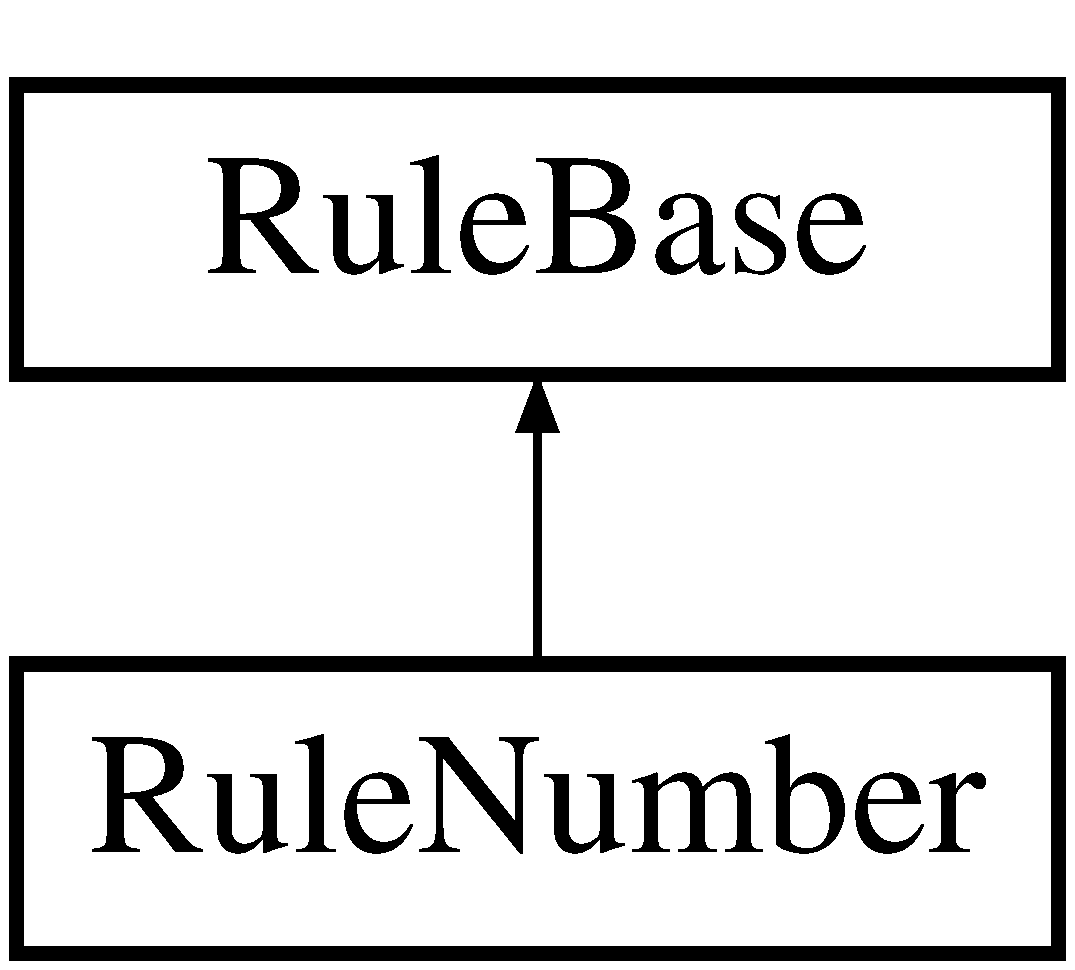
\includegraphics[height=2.000000cm]{class_rule_number}
\end{center}
\end{figure}
\subsection*{公開メンバ関数}
\begin{DoxyCompactItemize}
\item 
\hyperlink{class_rule_number_a095c5d389db211932136b53f25f39685}{\+\_\+\+\_\+construct} ()
\item 
\hyperlink{class_rule_number_afb0fafe7e02a3ae1993c01c19fad2bae}{run} ()
\end{DoxyCompactItemize}
\subsection*{その他の継承メンバ}


\subsection{詳解}
ルール:数値クラス

\begin{DoxyVersion}{バージョン}
1.\+0.\+0  U\+T\+F-\/8  2011/10/06  2011/10/19 
\end{DoxyVersion}
\begin{DoxyAuthor}{著者}
mamiya\+\_\+shou 
\end{DoxyAuthor}
\begin{DoxyCopyright}{著作権所有}
mamiya\+\_\+shou  M\+I\+T License  P\+H\+P 5.\+0 以上必須 
\end{DoxyCopyright}


\subsection{構築子と解体子}
\hypertarget{class_rule_number_a095c5d389db211932136b53f25f39685}{\index{Rule\+Number@{Rule\+Number}!\+\_\+\+\_\+construct@{\+\_\+\+\_\+construct}}
\index{\+\_\+\+\_\+construct@{\+\_\+\+\_\+construct}!Rule\+Number@{Rule\+Number}}
\subsubsection[{\+\_\+\+\_\+construct}]{\setlength{\rightskip}{0pt plus 5cm}\+\_\+\+\_\+construct (
\begin{DoxyParamCaption}
{}
\end{DoxyParamCaption}
)}}\label{class_rule_number_a095c5d389db211932136b53f25f39685}
コンストラクタ

public \begin{DoxyReturn}{戻り値}
void 
\end{DoxyReturn}


\subsection{関数詳解}
\hypertarget{class_rule_number_afb0fafe7e02a3ae1993c01c19fad2bae}{\index{Rule\+Number@{Rule\+Number}!run@{run}}
\index{run@{run}!Rule\+Number@{Rule\+Number}}
\subsubsection[{run}]{\setlength{\rightskip}{0pt plus 5cm}run (
\begin{DoxyParamCaption}
{}
\end{DoxyParamCaption}
)}}\label{class_rule_number_afb0fafe7e02a3ae1993c01c19fad2bae}
バリデートする

public \begin{DoxyReturn}{戻り値}
boolean T\+R\+U\+E(\+O\+K) / string エラーメッセージ(\+N\+G)  未入力('')の場合は\+T\+R\+U\+Eを返す 
\end{DoxyReturn}


このクラス詳解は次のファイルから抽出されました\+:\begin{DoxyCompactItemize}
\item 
Validate/rules/number.\+php\end{DoxyCompactItemize}

\hypertarget{class_rule_regular_expression}{\section{Rule\+Regular\+Expression クラス}
\label{class_rule_regular_expression}\index{Rule\+Regular\+Expression@{Rule\+Regular\+Expression}}
}
Rule\+Regular\+Expression の継承関係図\begin{figure}[H]
\begin{center}
\leavevmode
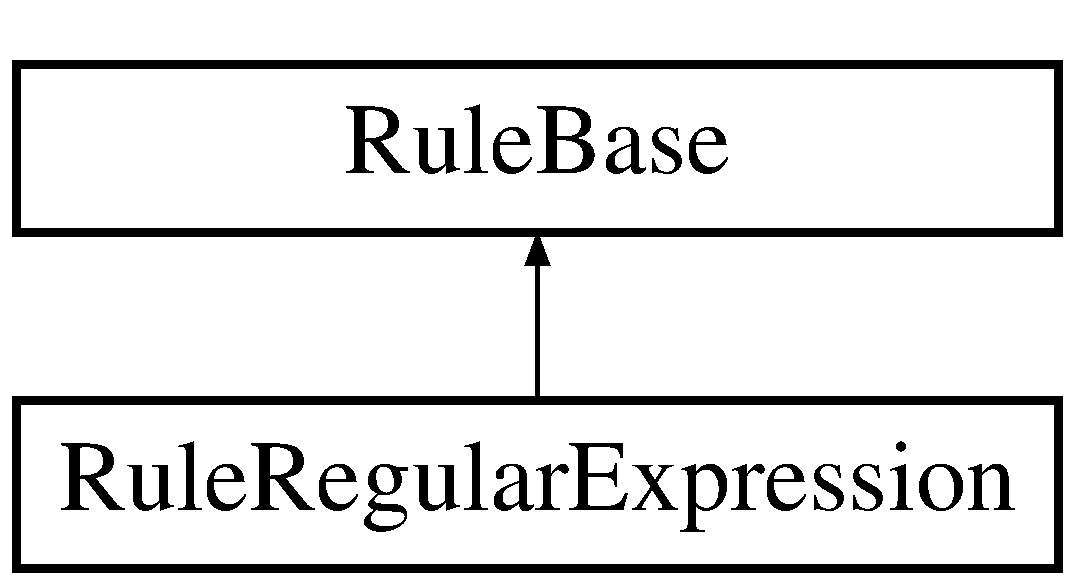
\includegraphics[height=2.000000cm]{class_rule_regular_expression}
\end{center}
\end{figure}
\subsection*{公開メンバ関数}
\begin{DoxyCompactItemize}
\item 
\hyperlink{class_rule_regular_expression_a095c5d389db211932136b53f25f39685}{\+\_\+\+\_\+construct} ()
\item 
\hyperlink{class_rule_regular_expression_afb0fafe7e02a3ae1993c01c19fad2bae}{run} ()
\end{DoxyCompactItemize}
\subsection*{その他の継承メンバ}


\subsection{詳解}
ルール:正規表現クラス

\begin{DoxyVersion}{バージョン}
1.\+0.\+0  U\+T\+F-\/8  2011/10/10  2011/10/19 
\end{DoxyVersion}
\begin{DoxyAuthor}{著者}
mamiya\+\_\+shou 
\end{DoxyAuthor}
\begin{DoxyCopyright}{著作権所有}
mamiya\+\_\+shou  M\+I\+T License  P\+H\+P 5.\+0 以上必須 
\end{DoxyCopyright}


\subsection{構築子と解体子}
\hypertarget{class_rule_regular_expression_a095c5d389db211932136b53f25f39685}{\index{Rule\+Regular\+Expression@{Rule\+Regular\+Expression}!\+\_\+\+\_\+construct@{\+\_\+\+\_\+construct}}
\index{\+\_\+\+\_\+construct@{\+\_\+\+\_\+construct}!Rule\+Regular\+Expression@{Rule\+Regular\+Expression}}
\subsubsection[{\+\_\+\+\_\+construct}]{\setlength{\rightskip}{0pt plus 5cm}\+\_\+\+\_\+construct (
\begin{DoxyParamCaption}
{}
\end{DoxyParamCaption}
)}}\label{class_rule_regular_expression_a095c5d389db211932136b53f25f39685}
コンストラクタ

public \begin{DoxyReturn}{戻り値}
void 
\end{DoxyReturn}


\subsection{関数詳解}
\hypertarget{class_rule_regular_expression_afb0fafe7e02a3ae1993c01c19fad2bae}{\index{Rule\+Regular\+Expression@{Rule\+Regular\+Expression}!run@{run}}
\index{run@{run}!Rule\+Regular\+Expression@{Rule\+Regular\+Expression}}
\subsubsection[{run}]{\setlength{\rightskip}{0pt plus 5cm}run (
\begin{DoxyParamCaption}
{}
\end{DoxyParamCaption}
)}}\label{class_rule_regular_expression_afb0fafe7e02a3ae1993c01c19fad2bae}
バリデートする

public \begin{DoxyReturn}{戻り値}
boolean T\+R\+U\+E(\+O\+K) / string エラーメッセージ(\+N\+G) 
\end{DoxyReturn}

\begin{DoxyExceptions}{例外}
{\em Exception} & validate.\+php \hyperlink{class_rule_regular_expression_afb0fafe7e02a3ae1993c01c19fad2bae}{run()}で捕捉する  未入力('')の場合は\+T\+R\+U\+Eを返す \\
\hline
\end{DoxyExceptions}


このクラス詳解は次のファイルから抽出されました\+:\begin{DoxyCompactItemize}
\item 
Validate/rules/regular\+\_\+expression.\+php\end{DoxyCompactItemize}

\hypertarget{class_rule_required}{\section{Rule\+Required クラス}
\label{class_rule_required}\index{Rule\+Required@{Rule\+Required}}
}
Rule\+Required の継承関係図\begin{figure}[H]
\begin{center}
\leavevmode
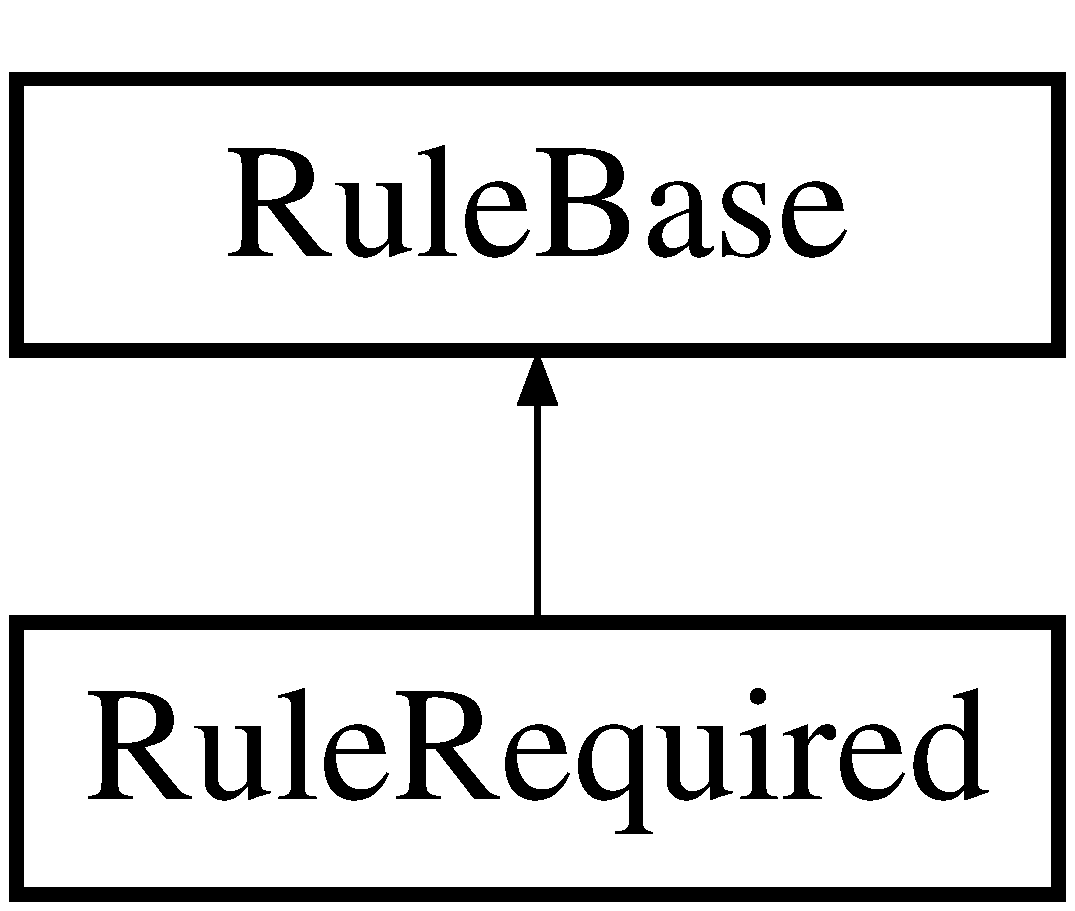
\includegraphics[height=2.000000cm]{class_rule_required}
\end{center}
\end{figure}
\subsection*{公開メンバ関数}
\begin{DoxyCompactItemize}
\item 
\hyperlink{class_rule_required_a095c5d389db211932136b53f25f39685}{\+\_\+\+\_\+construct} ()
\item 
\hyperlink{class_rule_required_afb0fafe7e02a3ae1993c01c19fad2bae}{run} ()
\end{DoxyCompactItemize}
\subsection*{その他の継承メンバ}


\subsection{詳解}
ルール:必須入力クラス

\begin{DoxyVersion}{バージョン}
1.\+0.\+0  U\+T\+F-\/8  2011/10/05  2011/10/19 
\end{DoxyVersion}
\begin{DoxyAuthor}{著者}
mamiya\+\_\+shou 
\end{DoxyAuthor}
\begin{DoxyCopyright}{著作権所有}
mamiya\+\_\+shou  M\+I\+T License  P\+H\+P 5.\+0 以上必須 
\end{DoxyCopyright}


\subsection{構築子と解体子}
\hypertarget{class_rule_required_a095c5d389db211932136b53f25f39685}{\index{Rule\+Required@{Rule\+Required}!\+\_\+\+\_\+construct@{\+\_\+\+\_\+construct}}
\index{\+\_\+\+\_\+construct@{\+\_\+\+\_\+construct}!Rule\+Required@{Rule\+Required}}
\subsubsection[{\+\_\+\+\_\+construct}]{\setlength{\rightskip}{0pt plus 5cm}\+\_\+\+\_\+construct (
\begin{DoxyParamCaption}
{}
\end{DoxyParamCaption}
)}}\label{class_rule_required_a095c5d389db211932136b53f25f39685}
コンストラクタ

public \begin{DoxyReturn}{戻り値}
void 
\end{DoxyReturn}


\subsection{関数詳解}
\hypertarget{class_rule_required_afb0fafe7e02a3ae1993c01c19fad2bae}{\index{Rule\+Required@{Rule\+Required}!run@{run}}
\index{run@{run}!Rule\+Required@{Rule\+Required}}
\subsubsection[{run}]{\setlength{\rightskip}{0pt plus 5cm}run (
\begin{DoxyParamCaption}
{}
\end{DoxyParamCaption}
)}}\label{class_rule_required_afb0fafe7e02a3ae1993c01c19fad2bae}
バリデートする

public \begin{DoxyReturn}{戻り値}
boolean T\+R\+U\+E(\+O\+K) / string エラーメッセージ(\+N\+G) 
\end{DoxyReturn}


このクラス詳解は次のファイルから抽出されました\+:\begin{DoxyCompactItemize}
\item 
Validate/rules/required.\+php\end{DoxyCompactItemize}

\hypertarget{class_rule_select}{\section{Rule\+Select クラス}
\label{class_rule_select}\index{Rule\+Select@{Rule\+Select}}
}
Rule\+Select の継承関係図\begin{figure}[H]
\begin{center}
\leavevmode
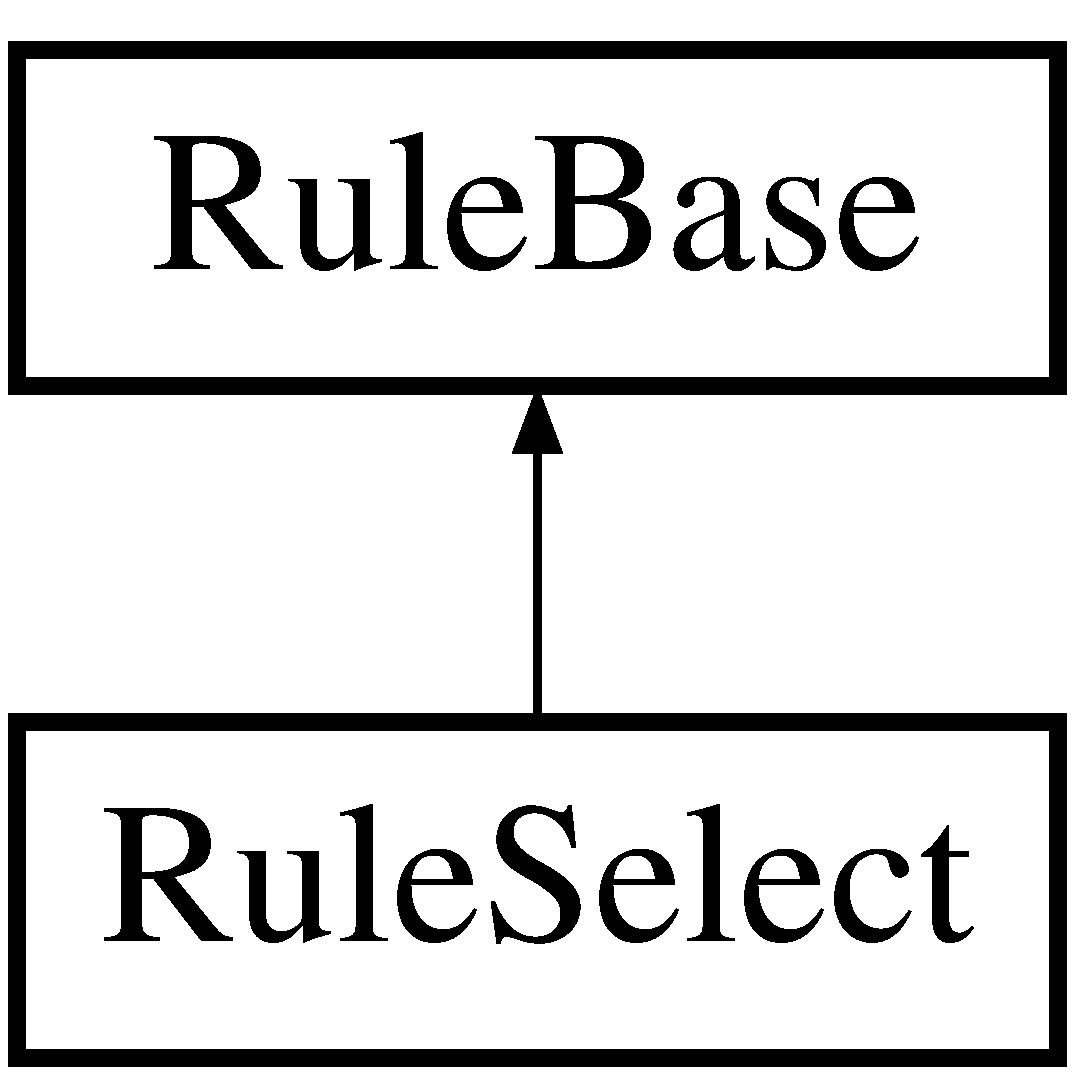
\includegraphics[height=2.000000cm]{class_rule_select}
\end{center}
\end{figure}
\subsection*{公開メンバ関数}
\begin{DoxyCompactItemize}
\item 
\hyperlink{class_rule_select_a095c5d389db211932136b53f25f39685}{\+\_\+\+\_\+construct} ()
\item 
\hyperlink{class_rule_select_afb0fafe7e02a3ae1993c01c19fad2bae}{run} ()
\end{DoxyCompactItemize}
\subsection*{その他の継承メンバ}


\subsection{詳解}
ルール:選択クラス

\begin{DoxyVersion}{バージョン}
1.\+0.\+0  U\+T\+F-\/8  2011/10/13  2011/10/19 
\end{DoxyVersion}
\begin{DoxyAuthor}{著者}
mamiya\+\_\+shou 
\end{DoxyAuthor}
\begin{DoxyCopyright}{著作権所有}
mamiya\+\_\+shou  M\+I\+T License 
\end{DoxyCopyright}


\subsection{構築子と解体子}
\hypertarget{class_rule_select_a095c5d389db211932136b53f25f39685}{\index{Rule\+Select@{Rule\+Select}!\+\_\+\+\_\+construct@{\+\_\+\+\_\+construct}}
\index{\+\_\+\+\_\+construct@{\+\_\+\+\_\+construct}!Rule\+Select@{Rule\+Select}}
\subsubsection[{\+\_\+\+\_\+construct}]{\setlength{\rightskip}{0pt plus 5cm}\+\_\+\+\_\+construct (
\begin{DoxyParamCaption}
{}
\end{DoxyParamCaption}
)}}\label{class_rule_select_a095c5d389db211932136b53f25f39685}
コンストラクタ

public \begin{DoxyReturn}{戻り値}
void 
\end{DoxyReturn}


\subsection{関数詳解}
\hypertarget{class_rule_select_afb0fafe7e02a3ae1993c01c19fad2bae}{\index{Rule\+Select@{Rule\+Select}!run@{run}}
\index{run@{run}!Rule\+Select@{Rule\+Select}}
\subsubsection[{run}]{\setlength{\rightskip}{0pt plus 5cm}run (
\begin{DoxyParamCaption}
{}
\end{DoxyParamCaption}
)}}\label{class_rule_select_afb0fafe7e02a3ae1993c01c19fad2bae}
バリデートする

public \begin{DoxyReturn}{戻り値}
boolean T\+R\+U\+E(\+O\+K) / string エラーメッセージ(\+N\+G) 
\end{DoxyReturn}

\begin{DoxyExceptions}{例外}
{\em Exception} & validate.\+php \hyperlink{class_rule_select_afb0fafe7e02a3ae1993c01c19fad2bae}{run()}で捕捉する \\
\hline
\end{DoxyExceptions}


このクラス詳解は次のファイルから抽出されました\+:\begin{DoxyCompactItemize}
\item 
Validate/rules/select.\+php\end{DoxyCompactItemize}

\hypertarget{class_rule_single}{\section{Rule\+Single クラス}
\label{class_rule_single}\index{Rule\+Single@{Rule\+Single}}
}
Rule\+Single の継承関係図\begin{figure}[H]
\begin{center}
\leavevmode
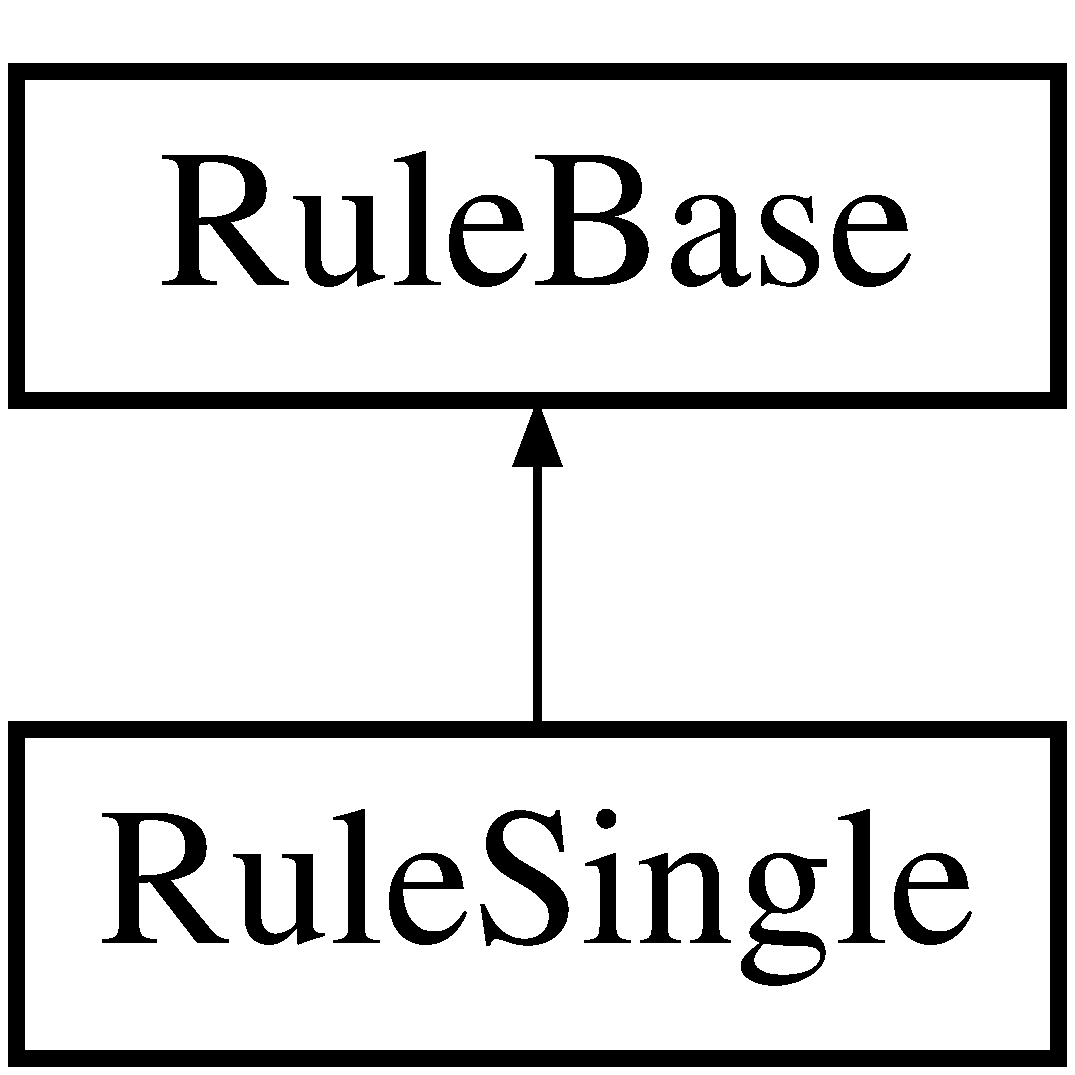
\includegraphics[height=2.000000cm]{class_rule_single}
\end{center}
\end{figure}
\subsection*{公開メンバ関数}
\begin{DoxyCompactItemize}
\item 
\hyperlink{class_rule_single_a095c5d389db211932136b53f25f39685}{\+\_\+\+\_\+construct} ()
\item 
\hyperlink{class_rule_single_afb0fafe7e02a3ae1993c01c19fad2bae}{run} ()
\end{DoxyCompactItemize}
\subsection*{その他の継承メンバ}


\subsection{詳解}
ルール:半角文字クラス

\begin{DoxyVersion}{バージョン}
1.\+0.\+0  U\+T\+F-\/8  2011/10/08  2011/10/19 
\end{DoxyVersion}
\begin{DoxyAuthor}{著者}
mamiya\+\_\+shou 
\end{DoxyAuthor}
\begin{DoxyCopyright}{著作権所有}
mamiya\+\_\+shou  M\+I\+T License  P\+H\+P 5.\+0 以上必須 
\end{DoxyCopyright}


\subsection{構築子と解体子}
\hypertarget{class_rule_single_a095c5d389db211932136b53f25f39685}{\index{Rule\+Single@{Rule\+Single}!\+\_\+\+\_\+construct@{\+\_\+\+\_\+construct}}
\index{\+\_\+\+\_\+construct@{\+\_\+\+\_\+construct}!Rule\+Single@{Rule\+Single}}
\subsubsection[{\+\_\+\+\_\+construct}]{\setlength{\rightskip}{0pt plus 5cm}\+\_\+\+\_\+construct (
\begin{DoxyParamCaption}
{}
\end{DoxyParamCaption}
)}}\label{class_rule_single_a095c5d389db211932136b53f25f39685}
コンストラクタ

public \begin{DoxyReturn}{戻り値}
void 
\end{DoxyReturn}


\subsection{関数詳解}
\hypertarget{class_rule_single_afb0fafe7e02a3ae1993c01c19fad2bae}{\index{Rule\+Single@{Rule\+Single}!run@{run}}
\index{run@{run}!Rule\+Single@{Rule\+Single}}
\subsubsection[{run}]{\setlength{\rightskip}{0pt plus 5cm}run (
\begin{DoxyParamCaption}
{}
\end{DoxyParamCaption}
)}}\label{class_rule_single_afb0fafe7e02a3ae1993c01c19fad2bae}
バリデートする

public \begin{DoxyReturn}{戻り値}
boolean T\+R\+U\+E(\+O\+K) / string エラーメッセージ(\+N\+G) 
\end{DoxyReturn}

\begin{DoxyExceptions}{例外}
{\em Exception} & validate.\+php \hyperlink{class_rule_single_afb0fafe7e02a3ae1993c01c19fad2bae}{run()}で捕捉する  未入力('')の場合は\+T\+R\+U\+Eを返す \\
\hline
\end{DoxyExceptions}


このクラス詳解は次のファイルから抽出されました\+:\begin{DoxyCompactItemize}
\item 
Validate/rules/single.\+php\end{DoxyCompactItemize}

\hypertarget{class_rule_tel}{\section{Rule\+Tel クラス}
\label{class_rule_tel}\index{Rule\+Tel@{Rule\+Tel}}
}
Rule\+Tel の継承関係図\begin{figure}[H]
\begin{center}
\leavevmode
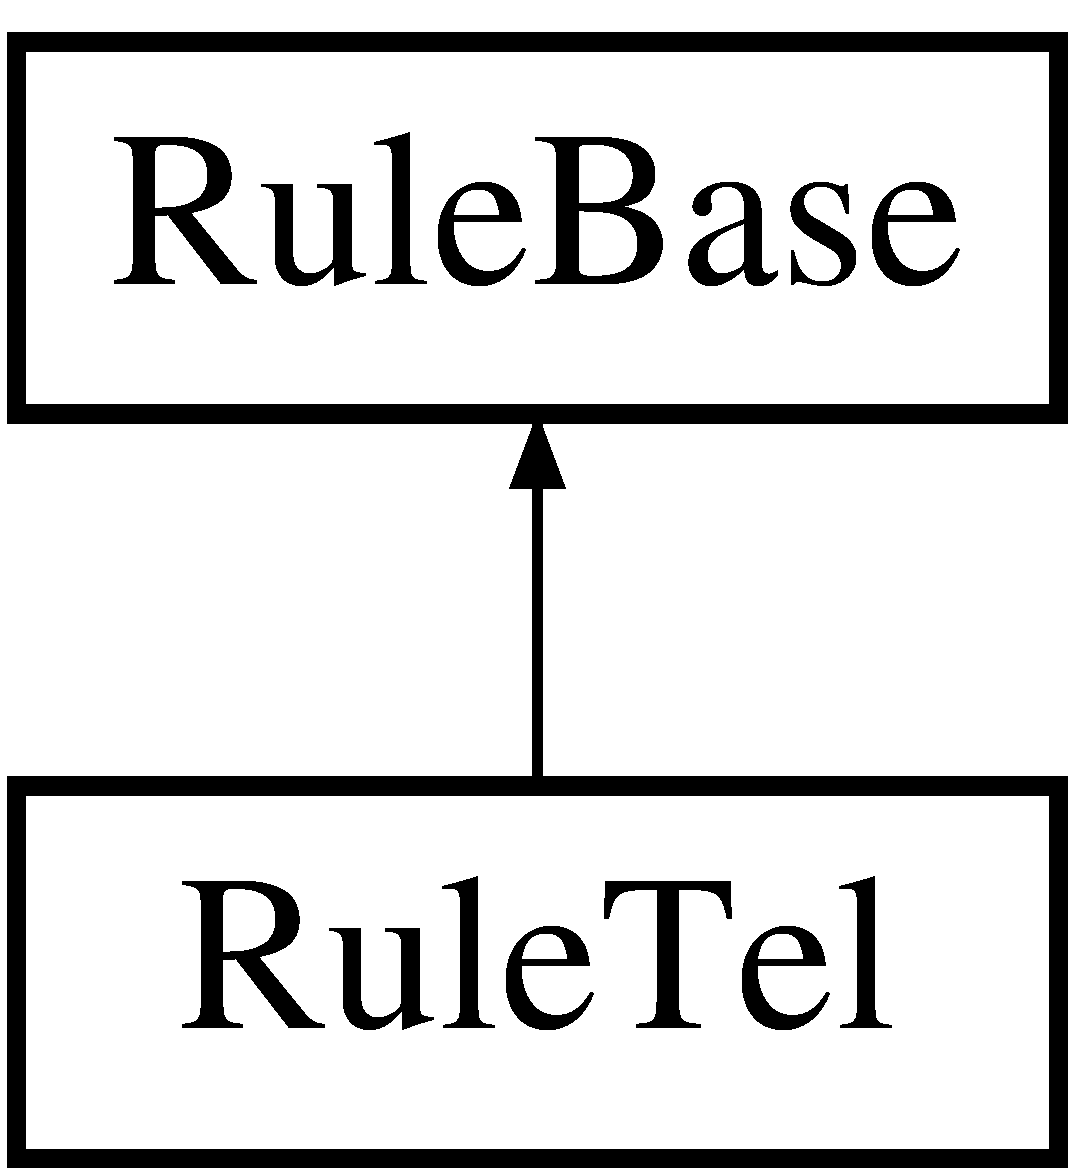
\includegraphics[height=2.000000cm]{class_rule_tel}
\end{center}
\end{figure}
\subsection*{公開メンバ関数}
\begin{DoxyCompactItemize}
\item 
\hyperlink{class_rule_tel_a095c5d389db211932136b53f25f39685}{\+\_\+\+\_\+construct} ()
\item 
\hyperlink{class_rule_tel_afb0fafe7e02a3ae1993c01c19fad2bae}{run} ()
\end{DoxyCompactItemize}
\subsection*{その他の継承メンバ}


\subsection{詳解}
ルール:電話番号クラス

\begin{DoxyVersion}{バージョン}
1.\+0.\+0  U\+T\+F-\/8  2011/10/09  2011/10/19 
\end{DoxyVersion}
\begin{DoxyAuthor}{著者}
mamiya\+\_\+shou 
\end{DoxyAuthor}
\begin{DoxyCopyright}{著作権所有}
mamiya\+\_\+shou  M\+I\+T License  P\+H\+P 5.\+0 以上必須 
\end{DoxyCopyright}


\subsection{構築子と解体子}
\hypertarget{class_rule_tel_a095c5d389db211932136b53f25f39685}{\index{Rule\+Tel@{Rule\+Tel}!\+\_\+\+\_\+construct@{\+\_\+\+\_\+construct}}
\index{\+\_\+\+\_\+construct@{\+\_\+\+\_\+construct}!Rule\+Tel@{Rule\+Tel}}
\subsubsection[{\+\_\+\+\_\+construct}]{\setlength{\rightskip}{0pt plus 5cm}\+\_\+\+\_\+construct (
\begin{DoxyParamCaption}
{}
\end{DoxyParamCaption}
)}}\label{class_rule_tel_a095c5d389db211932136b53f25f39685}
コンストラクタ

public \begin{DoxyReturn}{戻り値}
void 
\end{DoxyReturn}


\subsection{関数詳解}
\hypertarget{class_rule_tel_afb0fafe7e02a3ae1993c01c19fad2bae}{\index{Rule\+Tel@{Rule\+Tel}!run@{run}}
\index{run@{run}!Rule\+Tel@{Rule\+Tel}}
\subsubsection[{run}]{\setlength{\rightskip}{0pt plus 5cm}run (
\begin{DoxyParamCaption}
{}
\end{DoxyParamCaption}
)}}\label{class_rule_tel_afb0fafe7e02a3ae1993c01c19fad2bae}
バリデートする

public \begin{DoxyReturn}{戻り値}
boolean T\+R\+U\+E(\+O\+K) / string エラーメッセージ(\+N\+G) 
\end{DoxyReturn}

\begin{DoxyExceptions}{例外}
{\em Exception} & validate.\+php \hyperlink{class_rule_tel_afb0fafe7e02a3ae1993c01c19fad2bae}{run()}で捕捉する  未入力('')の場合は\+T\+R\+U\+Eを返す \\
\hline
\end{DoxyExceptions}


このクラス詳解は次のファイルから抽出されました\+:\begin{DoxyCompactItemize}
\item 
Validate/rules/tel.\+php\end{DoxyCompactItemize}

\hypertarget{class_rule_time}{\section{Rule\+Time クラス}
\label{class_rule_time}\index{Rule\+Time@{Rule\+Time}}
}
Rule\+Time の継承関係図\begin{figure}[H]
\begin{center}
\leavevmode
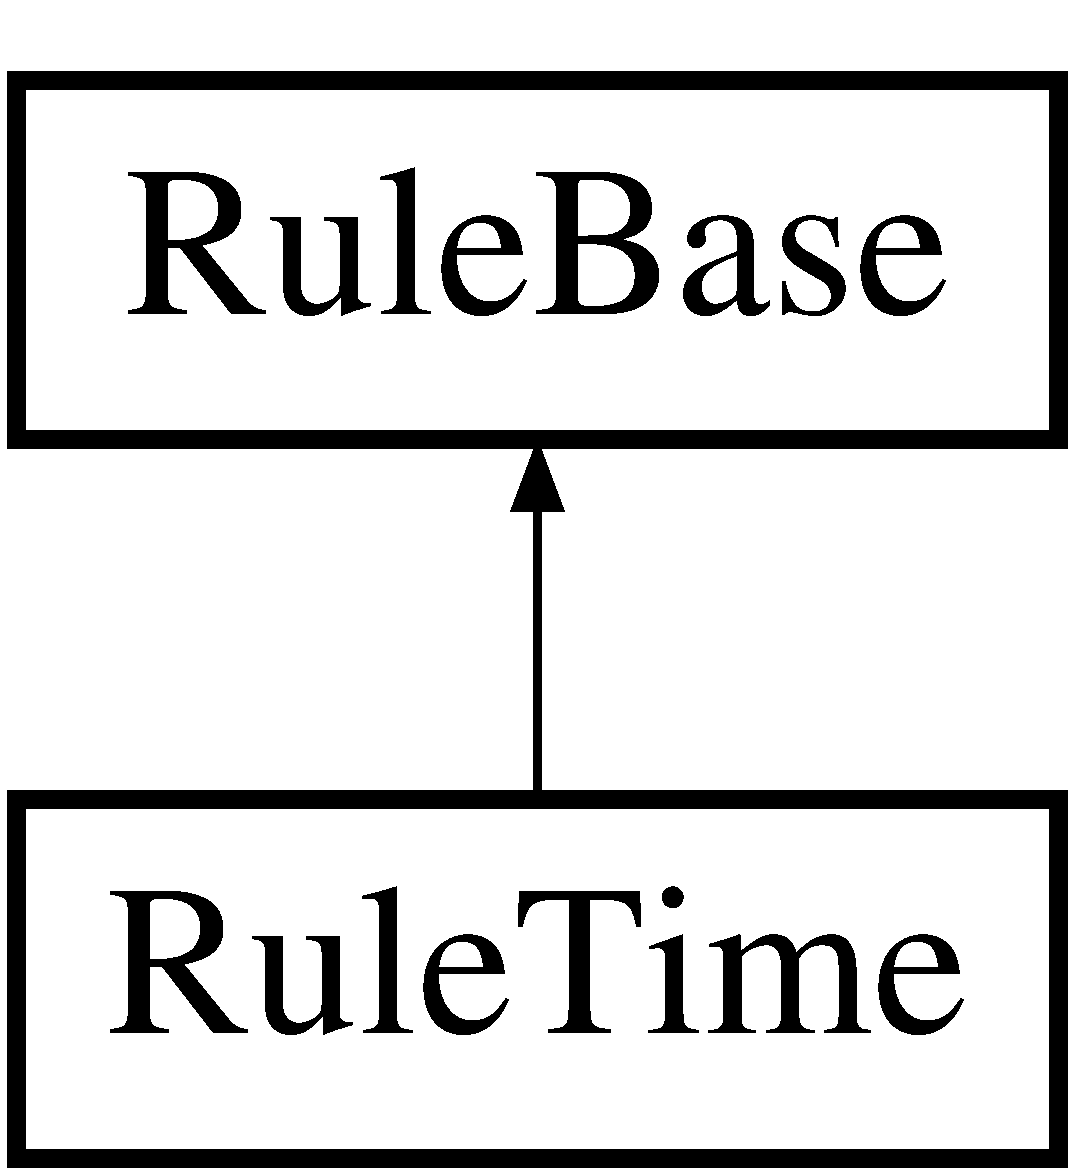
\includegraphics[height=2.000000cm]{class_rule_time}
\end{center}
\end{figure}
\subsection*{公開メンバ関数}
\begin{DoxyCompactItemize}
\item 
\hyperlink{class_rule_time_a095c5d389db211932136b53f25f39685}{\+\_\+\+\_\+construct} ()
\item 
\hyperlink{class_rule_time_afb0fafe7e02a3ae1993c01c19fad2bae}{run} ()
\end{DoxyCompactItemize}
\subsection*{その他の継承メンバ}


\subsection{詳解}
ルール:時刻クラス

\begin{DoxyVersion}{バージョン}
1.\+0.\+0  U\+T\+F-\/8  2011/10/11  2011/10/19 
\end{DoxyVersion}
\begin{DoxyAuthor}{著者}
mamiya\+\_\+shou 
\end{DoxyAuthor}
\begin{DoxyCopyright}{著作権所有}
mamiya\+\_\+shou  M\+I\+T License  P\+H\+P 5.\+0 以上必須 
\end{DoxyCopyright}


\subsection{構築子と解体子}
\hypertarget{class_rule_time_a095c5d389db211932136b53f25f39685}{\index{Rule\+Time@{Rule\+Time}!\+\_\+\+\_\+construct@{\+\_\+\+\_\+construct}}
\index{\+\_\+\+\_\+construct@{\+\_\+\+\_\+construct}!Rule\+Time@{Rule\+Time}}
\subsubsection[{\+\_\+\+\_\+construct}]{\setlength{\rightskip}{0pt plus 5cm}\+\_\+\+\_\+construct (
\begin{DoxyParamCaption}
{}
\end{DoxyParamCaption}
)}}\label{class_rule_time_a095c5d389db211932136b53f25f39685}
コンストラクタ

public \begin{DoxyReturn}{戻り値}
void 
\end{DoxyReturn}


\subsection{関数詳解}
\hypertarget{class_rule_time_afb0fafe7e02a3ae1993c01c19fad2bae}{\index{Rule\+Time@{Rule\+Time}!run@{run}}
\index{run@{run}!Rule\+Time@{Rule\+Time}}
\subsubsection[{run}]{\setlength{\rightskip}{0pt plus 5cm}run (
\begin{DoxyParamCaption}
{}
\end{DoxyParamCaption}
)}}\label{class_rule_time_afb0fafe7e02a3ae1993c01c19fad2bae}
バリデートする

public \begin{DoxyReturn}{戻り値}
boolean T\+R\+U\+E(\+O\+K) / string エラーメッセージ(\+N\+G) 
\end{DoxyReturn}

\begin{DoxyExceptions}{例外}
{\em Exception} & validate.\+php \hyperlink{class_rule_time_afb0fafe7e02a3ae1993c01c19fad2bae}{run()}で捕捉する  未入力('')の場合は\+T\+R\+U\+Eを返す \\
\hline
\end{DoxyExceptions}


このクラス詳解は次のファイルから抽出されました\+:\begin{DoxyCompactItemize}
\item 
Validate/rules/time.\+php\end{DoxyCompactItemize}

\hypertarget{class_rule_zip}{\section{Rule\+Zip クラス}
\label{class_rule_zip}\index{Rule\+Zip@{Rule\+Zip}}
}
Rule\+Zip の継承関係図\begin{figure}[H]
\begin{center}
\leavevmode
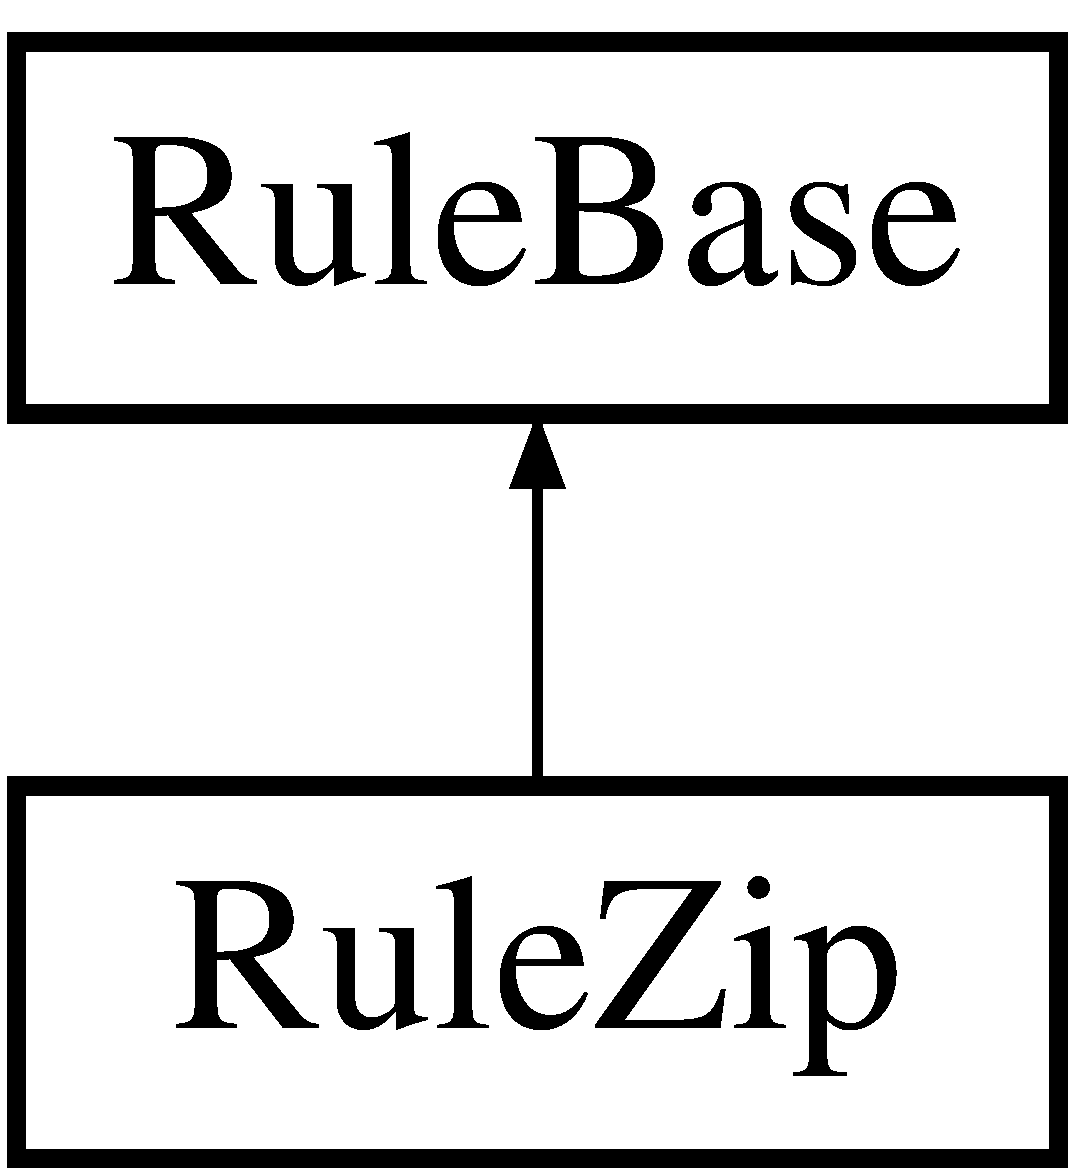
\includegraphics[height=2.000000cm]{class_rule_zip}
\end{center}
\end{figure}
\subsection*{公開メンバ関数}
\begin{DoxyCompactItemize}
\item 
\hyperlink{class_rule_zip_a095c5d389db211932136b53f25f39685}{\+\_\+\+\_\+construct} ()
\item 
\hyperlink{class_rule_zip_afb0fafe7e02a3ae1993c01c19fad2bae}{run} ()
\end{DoxyCompactItemize}
\subsection*{フィールド}
\begin{DoxyCompactItemize}
\item 
\hypertarget{class_rule_zip_ab168cbeba579bbfed03fe9f7b039d3ee}{const {\bfseries Z\+I\+P\+\_\+\+F\+I\+L\+E} = 'zip/Zip.\+php'}\label{class_rule_zip_ab168cbeba579bbfed03fe9f7b039d3ee}

\end{DoxyCompactItemize}
\subsection*{その他の継承メンバ}


\subsection{詳解}
ルール:郵便番号クラス

\begin{DoxyVersion}{バージョン}
1.\+0.\+0  U\+T\+F-\/8  2011/10/10  2011/10/19 
\end{DoxyVersion}
\begin{DoxyAuthor}{著者}
mamiya\+\_\+shou 
\end{DoxyAuthor}
\begin{DoxyCopyright}{著作権所有}
mamiya\+\_\+shou  M\+I\+T License  P\+H\+P 5.\+0 以上必須 
\end{DoxyCopyright}


\subsection{構築子と解体子}
\hypertarget{class_rule_zip_a095c5d389db211932136b53f25f39685}{\index{Rule\+Zip@{Rule\+Zip}!\+\_\+\+\_\+construct@{\+\_\+\+\_\+construct}}
\index{\+\_\+\+\_\+construct@{\+\_\+\+\_\+construct}!Rule\+Zip@{Rule\+Zip}}
\subsubsection[{\+\_\+\+\_\+construct}]{\setlength{\rightskip}{0pt plus 5cm}\+\_\+\+\_\+construct (
\begin{DoxyParamCaption}
{}
\end{DoxyParamCaption}
)}}\label{class_rule_zip_a095c5d389db211932136b53f25f39685}
コンストラクタ

public \begin{DoxyReturn}{戻り値}
void 
\end{DoxyReturn}


\subsection{関数詳解}
\hypertarget{class_rule_zip_afb0fafe7e02a3ae1993c01c19fad2bae}{\index{Rule\+Zip@{Rule\+Zip}!run@{run}}
\index{run@{run}!Rule\+Zip@{Rule\+Zip}}
\subsubsection[{run}]{\setlength{\rightskip}{0pt plus 5cm}run (
\begin{DoxyParamCaption}
{}
\end{DoxyParamCaption}
)}}\label{class_rule_zip_afb0fafe7e02a3ae1993c01c19fad2bae}
バリデートする

public \begin{DoxyReturn}{戻り値}
boolean T\+R\+U\+E(\+O\+K) / string エラーメッセージ(\+N\+G)  未入力('')の場合は\+T\+R\+U\+Eを返す 
\end{DoxyReturn}


このクラス詳解は次のファイルから抽出されました\+:\begin{DoxyCompactItemize}
\item 
Validate/rules/zip.\+php\end{DoxyCompactItemize}

\hypertarget{class_validate}{\section{Validate クラス}
\label{class_validate}\index{Validate@{Validate}}
}
\subsection*{公開メンバ関数}
\begin{DoxyCompactItemize}
\item 
\hyperlink{class_validate_affd2166b9ae24d7f6d972b6e8e27ab64}{\+\_\+\+\_\+construct} (\$requests)
\item 
\hyperlink{class_validate_a0f28658da9689c7abbfeef6620621b11}{add\+Rule} ()
\item 
\hyperlink{class_validate_a3784964295510f2bf9e3c08945073a6e}{del\+Rule} (\$name, \$type=N\+U\+L\+L)
\item 
\hyperlink{class_validate_afc81a53f0add88b49c6f84068d47987b}{copy\+Rule} (\$dest\+Name, \$src\+Name)
\item 
\hyperlink{class_validate_afb0fafe7e02a3ae1993c01c19fad2bae}{run} ()
\end{DoxyCompactItemize}
\subsection*{フィールド}
\begin{DoxyCompactItemize}
\item 
\hypertarget{class_validate_ab24faf4aa647cdcee494fc48524ad4ff}{{\bfseries \$errors}}\label{class_validate_ab24faf4aa647cdcee494fc48524ad4ff}

\item 
\hypertarget{class_validate_a233d12bd8b6d3453e9a7a3f0b8c31db2}{{\bfseries \$results}}\label{class_validate_a233d12bd8b6d3453e9a7a3f0b8c31db2}

\end{DoxyCompactItemize}


\subsection{詳解}
バリデートクラス

\begin{DoxyVersion}{バージョン}
1.\+0.\+0  U\+T\+F-\/8  2011/10/05  2011/10/19 
\end{DoxyVersion}
\begin{DoxyAuthor}{著者}
mamiya\+\_\+shou 
\end{DoxyAuthor}
\begin{DoxyCopyright}{著作権所有}
mamiya\+\_\+shou  M\+I\+T License  P\+H\+P 5.\+0 以上必須 
\end{DoxyCopyright}


\subsection{構築子と解体子}
\hypertarget{class_validate_affd2166b9ae24d7f6d972b6e8e27ab64}{\index{Validate@{Validate}!\+\_\+\+\_\+construct@{\+\_\+\+\_\+construct}}
\index{\+\_\+\+\_\+construct@{\+\_\+\+\_\+construct}!Validate@{Validate}}
\subsubsection[{\+\_\+\+\_\+construct}]{\setlength{\rightskip}{0pt plus 5cm}\+\_\+\+\_\+construct (
\begin{DoxyParamCaption}
\item[{}]{\$requests}
\end{DoxyParamCaption}
)}}\label{class_validate_affd2166b9ae24d7f6d972b6e8e27ab64}
コンストラクタ

public 
\begin{DoxyParams}[1]{引数}
array & {\em \$posts} & リクエスト配列 \\
\hline
\end{DoxyParams}
\begin{DoxyReturn}{戻り値}
void 
\end{DoxyReturn}


\subsection{関数詳解}
\hypertarget{class_validate_a0f28658da9689c7abbfeef6620621b11}{\index{Validate@{Validate}!add\+Rule@{add\+Rule}}
\index{add\+Rule@{add\+Rule}!Validate@{Validate}}
\subsubsection[{add\+Rule}]{\setlength{\rightskip}{0pt plus 5cm}add\+Rule (
\begin{DoxyParamCaption}
{}
\end{DoxyParamCaption}
)}}\label{class_validate_a0f28658da9689c7abbfeef6620621b11}
ルールを追加する

public 
\begin{DoxyParams}{引数}
{\em 可変長引数(name,type} & \mbox{[}, etc \mbox{[}, etc...\mbox{]}\mbox{]}) \\
\hline
\end{DoxyParams}
\begin{DoxyReturn}{戻り値}
boolean T\+R\+U\+E(\+O\+K) / F\+A\+L\+S\+E(\+N\+G) 
\end{DoxyReturn}
\hypertarget{class_validate_afc81a53f0add88b49c6f84068d47987b}{\index{Validate@{Validate}!copy\+Rule@{copy\+Rule}}
\index{copy\+Rule@{copy\+Rule}!Validate@{Validate}}
\subsubsection[{copy\+Rule}]{\setlength{\rightskip}{0pt plus 5cm}copy\+Rule (
\begin{DoxyParamCaption}
\item[{}]{\$dest\+Name, }
\item[{}]{\$src\+Name}
\end{DoxyParamCaption}
)}}\label{class_validate_afc81a53f0add88b49c6f84068d47987b}
ルールをコピーする

public 
\begin{DoxyParams}[1]{引数}
string & {\em \$dest\+Name} & コピー先のname値 \\
\hline
string & {\em \$src\+Name} & コピー元のname値 \\
\hline
\end{DoxyParams}
\begin{DoxyReturn}{戻り値}
boolean T\+R\+U\+E(\+O\+K) / F\+A\+L\+S\+E(\+N\+G) 
\end{DoxyReturn}
\hypertarget{class_validate_a3784964295510f2bf9e3c08945073a6e}{\index{Validate@{Validate}!del\+Rule@{del\+Rule}}
\index{del\+Rule@{del\+Rule}!Validate@{Validate}}
\subsubsection[{del\+Rule}]{\setlength{\rightskip}{0pt plus 5cm}del\+Rule (
\begin{DoxyParamCaption}
\item[{}]{\$name, }
\item[{}]{\$type = {\ttfamily NULL}}
\end{DoxyParamCaption}
)}}\label{class_validate_a3784964295510f2bf9e3c08945073a6e}
ルールを削除する

public 
\begin{DoxyParams}[1]{引数}
string & {\em \$name} & name値 \\
\hline
string & {\em \$type} & ルール名 \\
\hline
\end{DoxyParams}
\begin{DoxyReturn}{戻り値}
boolean T\+R\+U\+E(\+O\+K) / F\+A\+L\+S\+E(\+N\+G) 
\end{DoxyReturn}
\hypertarget{class_validate_afb0fafe7e02a3ae1993c01c19fad2bae}{\index{Validate@{Validate}!run@{run}}
\index{run@{run}!Validate@{Validate}}
\subsubsection[{run}]{\setlength{\rightskip}{0pt plus 5cm}run (
\begin{DoxyParamCaption}
{}
\end{DoxyParamCaption}
)}}\label{class_validate_afb0fafe7e02a3ae1993c01c19fad2bae}
バリデーションを実行する

public \begin{DoxyReturn}{戻り値}
boolean T\+R\+U\+E(エラー無し) / F\+A\+L\+S\+E(エラー有り) 
\end{DoxyReturn}


このクラス詳解は次のファイルから抽出されました\+:\begin{DoxyCompactItemize}
\item 
Validate/Validate.\+php\end{DoxyCompactItemize}

\hypertarget{class_zip}{\section{Zip クラス}
\label{class_zip}\index{Zip@{Zip}}
}
\subsection*{静的公開メンバ関数}
\begin{DoxyCompactItemize}
\item 
static \hyperlink{class_zip_a5a1e04dc6e1e26996d8c398666f59f62}{search} (\$zip, \$is\+New=T\+R\+U\+E)
\end{DoxyCompactItemize}


\subsection{関数詳解}
\hypertarget{class_zip_a5a1e04dc6e1e26996d8c398666f59f62}{\index{Zip@{Zip}!search@{search}}
\index{search@{search}!Zip@{Zip}}
\subsubsection[{search}]{\setlength{\rightskip}{0pt plus 5cm}static search (
\begin{DoxyParamCaption}
\item[{}]{\$zip, }
\item[{}]{\$is\+New = {\ttfamily TRUE}}
\end{DoxyParamCaption}
)\hspace{0.3cm}{\ttfamily [static]}}}\label{class_zip_a5a1e04dc6e1e26996d8c398666f59f62}
郵便番号検索を行う


\begin{DoxyParams}[1]{引数}
string & {\em \$zip} & 郵便番号 \\
\hline
boolean & {\em \$is\+New} & true \+:現行郵便番号(7桁) false \+:旧式郵便番号(3桁 or 5桁) \\
\hline
\end{DoxyParams}
\begin{DoxyReturn}{戻り値}
boolean 結果オブジェクト配列(\+O\+K) / F\+A\+L\+S\+E(\+N\+G) 
\end{DoxyReturn}


このクラス詳解は次のファイルから抽出されました\+:\begin{DoxyCompactItemize}
\item 
Validate/rules/zip/Zip.\+php\end{DoxyCompactItemize}

%--- End generated contents ---

% Index
\newpage
\phantomsection
\addcontentsline{toc}{chapter}{索引}
\printindex

\end{document}
